% Options for packages loaded elsewhere
\PassOptionsToPackage{unicode}{hyperref}
\PassOptionsToPackage{hyphens}{url}
\documentclass{article}
\usepackage[a4paper,margin=1in]{geometry}
\usepackage{xcolor}
\usepackage{amsmath,amssymb}
\setcounter{secnumdepth}{3}
\usepackage{iftex}
\ifPDFTeX
  \usepackage[T1]{fontenc}
  \usepackage[utf8]{inputenc}
  \usepackage{textcomp} % provide euro and other symbols
  \usepackage{newunicodechar}
  \newunicodechar{≥}{\ensuremath{\ge}}
  \newunicodechar{≈}{\ensuremath{\approx}}
  \newunicodechar{▼}{\texttt{v}}
  \newunicodechar{─}{\texttt{-}}
  \newunicodechar{│}{\texttt{|}}
  \newunicodechar{┌}{\texttt{+}}
  \newunicodechar{┐}{\texttt{+}}
  \newunicodechar{└}{\texttt{+}}
  \newunicodechar{┘}{\texttt{+}}
  \newunicodechar{├}{\texttt{+}}
  \newunicodechar{┬}{\texttt{+}}
  \newunicodechar{┼}{\texttt{+}}
\else % if luatex or xetex
  \usepackage{unicode-math} % this also loads fontspec
  \defaultfontfeatures{Scale=MatchLowercase}
  \defaultfontfeatures[\rmfamily]{Ligatures=TeX,Scale=1}
\fi
\usepackage{lmodern}
\ifPDFTeX\else
  % xetex/luatex font selection
\fi
\IfFileExists{upquote.sty}{\usepackage{upquote}}{}
\IfFileExists{microtype.sty}{%
  \usepackage[]{microtype}
  \UseMicrotypeSet[protrusion]{basicmath}
}{}
\makeatletter
\@ifundefined{KOMAClassName}{%
  \IfFileExists{parskip.sty}{%
    \usepackage{parskip}
  }{%
    \setlength{\parindent}{0pt}
    \setlength{\parskip}{6pt plus 2pt minus 1pt}}
}{%
  \KOMAoptions{parskip=half}}
\makeatother
\setlength{\parindent}{0pt}
\setlength{\parskip}{0.8em}
\raggedbottom
\usepackage{longtable,booktabs,array}
\usepackage{calc}
\usepackage{tikz}
\usetikzlibrary{positioning,arrows.meta}
\usepackage{etoolbox}
\makeatletter
\patchcmd\longtable{\par}{\if@noskipsec\mbox{}\fi\par}{}{}
\makeatother
\IfFileExists{footnotehyper.sty}{\usepackage{footnotehyper}}{\usepackage{footnote}}
\makesavenoteenv{longtable}
\makeatletter
\renewcommand*\theHLT@tables{\thepage.\arabic{LT@tables}}
\makeatother
\setlength{\emergencystretch}{3em}
\hbadness=10000
\hfuzz=100pt
\providecommand{\tightlist}{%
  \setlength{\itemsep}{0pt}\setlength{\parskip}{0.8em}}
\usepackage{bookmark}
\usepackage{fvextra}
\DefineVerbatimEnvironment{verbatim}{Verbatim}{breaklines=true,breakanywhere=true}
\usepackage{csquotes}
\usepackage[backend=biber,style=authoryear]{biblatex}
\addbibresource{reference.bib}
\IfFileExists{xurl.sty}{\usepackage{xurl}}{}
\urlstyle{same}
\hypersetup{
  pdftitle={A Reproduction Study of Agent Workflow Memory on Mind2Web},
  hidelinks,
  pdfcreator={LaTeX via pandoc}}
\ifdefined\pdfsuppresswarningdupdest\pdfsuppresswarningdupdest=1\fi

\title{A Reproduction Study of Agent Workflow Memory on Mind2Web}
\author{Li Mengxiao}
\date{April 2026}

\begin{document}
\maketitle
\tableofcontents
\newpage

\section*{Abstract}\addcontentsline{toc}{section}{Abstract}

Agent Workflow Memory (AWM) is a representative approach for equipping
LLM-based web agents with reusable procedural knowledge extracted from
past trajectories. The original paper presents AWM as a broadly
effective memory mechanism, reporting substantial gains on Mind2Web and
WebArena and emphasizing the value of abstract LM-induced workflows.
We present a \textbf{Mind2Web-focused reproduction study} of AWM with
step-level and case-level analysis. The study is deliberately bounded
to a specific experimental envelope: Mind2Web only, first-run results,
GPT-4o and Qwen-3.5-397B-A17B as backbones (rather than the paper's
GPT-4 and GPT-3.5-turbo), and the released Mind2Web pipeline as
implemented. The
findings should therefore be read as setting-specific rather than as
model-agnostic or repeated-trial conclusions. Rather than stopping at
aggregate score comparison, the study evaluates the paper's main
Mind2Web claims and then traces the method's effects through
step-level decomposition, a 475-step paired-case analysis, target-site
result tracing in the online generalization setting, workflow text
comparison, and manually verified prompt-level case studies.

The strongest support is found for the paper's \textbf{mechanistic}
claims rather than its broadest \textbf{performance} claims. In the
current first-run setting, we find direct support that LM-induced
workflows are more abstract than rule-induced workflows at the text
level, that prompt-level code and text workflows behave similarly on
the audited site, and that induced workflow libraries are compact and
low-overlap. In contrast, in our first-run evidence, offline AWM is
mixed rather than uniformly superior across seven sites, online AWM
does not become stronger under larger distribution shift, and the claim
that natural-language observations are generally better than HTML is not
supported in the three-site evaluation.

The main contribution of this report is to explain \textbf{why} AWM
helps on some sites and harms on others. On positive-outcome sites,
workflow produces zero negative interventions; on negative-outcome
sites, negative interventions substantially outnumber positive ones.
AWM's actual
influence window is narrow, changing behavior on only 6--18\% of steps
through specific mechanisms: strategy redirection, value format
correction, and premature termination prevention on matched sites;
domain misdirection, template step-skipping, and apparent
workflow-first behavior on mismatched sites. We tentatively identify
eight recurring boundary-condition patterns not discussed in the
original paper and summarize a mechanism-consistent interpretive
framework connecting workflow induction quality, task-workflow semantic
match, and sparse step-level intervention to aggregate outcomes.

Read against the Interim report's gap analysis, this makes AWM a
representative but incomplete answer to procedural memory for GUI
agents: it operationalizes post-task workflow reuse, but does not yet
establish robust coverage across sites or a mechanism for failure-driven
revision.

The most defensible conclusion is that, under the present experimental
envelope (Mind2Web only, first-run, GPT-4o and Qwen-3.5-397B-A17B,
released-code-faithful pipeline), AWM is best understood as a
\textbf{conditionally effective prompting mechanism} rather than a
uniformly reliable memory method. Its core idea survives reproduction
better than its strongest performance narrative, but the present
evidence neither isolates method effects from backbone effects nor
substitutes for repeated-trial validation.

\section{Introduction}\label{introduction}

\subsection{Background}\label{background}

Large language model web agents often solve tasks in a stateless manner:
each episode is treated as independent, and the agent discards the
procedural patterns it just discovered. Human web users, by contrast,
accumulate reusable know-how: where search boxes usually live, how date
selection interfaces behave, when to browse versus when to search, and
how to recognize repeated UI motifs.

Agent Workflow Memory (AWM), proposed by \textcite{wang2024agent}, aims to
endow web agents with this kind of reusable procedural guidance. The
core idea is simple: induce workflows from successful trajectories,
store them as reusable memory, and inject them back into the prompt on
future tasks. The paper evaluates AWM in two modes:

\begin{itemize}
\tightlist
\item
  \textbf{Offline AWM}, where workflows are induced from annotated
  training examples before test time.
\item
  \textbf{Online AWM}, where workflows are induced incrementally from
  the agent's own successful test-time trajectories in a streaming
  fashion.
\end{itemize}

The original paper reports a 24.6\% relative improvement in step success
rate on Mind2Web and a 51.1\% relative improvement in task success rate
on WebArena, with further gains under cross-website and cross-domain
generalization.

\subsection{Framing: From the Interim Gap Analysis to This
Reproduction}\label{framing-from-the-interim-gap-analysis-to-this-reproduction}

The Interim report identified two especially load-bearing gaps for
GUI-agent research: reusable procedural memory and failure-driven
write-back. AWM is a natural focal case for the present final report
because it is a representative attempt to operationalize the first of
these gaps through post-task workflow induction and cross-task prompt
reuse.

That makes AWM a suitable system for a guided-study final report.
Before proposing a new memory architecture, it is more informative to
audit how far a representative workflow-memory system already goes:
whether it materially covers the procedural-memory problem, what
mechanisms produce any gains, and which boundary conditions expose the
still-missing failure-driven revision component. The report is therefore
intentionally narrow in system scope and deep in evidence structure.

\subsection{Why Deep Reproduction Is
Needed}\label{why-deep-reproduction-is-needed}

For AWM, a shallow reproduction would be inadequate. Matching a few
aggregate numbers cannot answer the most important questions:

\begin{enumerate}
\def\labelenumi{\arabic{enumi}.}
\tightlist
\item
  Does the method really work across tasks, websites, and domains?
\item
  If it works, what exact step-level mechanism produces the gains?
\item
  If it fails, under what boundary conditions does it fail?
\end{enumerate}

These are especially important because AWM makes several ambitious
claims at once:

\begin{itemize}
\tightlist
\item
  Workflows can be abstracted from experience.
\item
  Those workflows transfer across related tasks.
\item
  Online induction becomes especially useful under larger distribution
  shift.
\item
  Natural-language environment descriptions outperform HTML.
\item
  Compact workflow libraries can still be highly useful.
\end{itemize}

We therefore adopt a deeper reproduction strategy: first verify the main
claims, then explain the mechanisms, and finally identify the boundary
conditions.

\subsection{Research Objectives}\label{research-objectives}

Our study proceeds in three stages:

\begin{itemize}
\tightlist
\item
  \textbf{Layer 1: Reproduction of Main Claims.} Do the paper's main
  Mind2Web claims hold under independent reproduction?
\item
  \textbf{Layer 2: Mechanism Explanation.} Through what specific
  mechanisms does AWM improve or degrade step-level agent behavior?
\item
  \textbf{Layer 3: Boundary Identification.} What trade-offs, failure
  modes, and conditional patterns are left unclear or unreported in the
  original paper?
\end{itemize}

\subsection{Scope}\label{scope}

This study is restricted to \textbf{Mind2Web} and reports
\textbf{first-run results only}.

\begin{itemize}
\tightlist
\item
  The main evidence base is \textbf{Mind2Web only}.
\item
  All positive / negative / mixed judgments are \textbf{first-run
  judgments}.
\item
  The paper's \texttt{AWM\_AS} action-space extension experiment is
  \textbf{not covered}.
\item
  Alignment-rate analysis is used only as an \textbf{exploratory
  heuristic}, not as a strong semantic metric.
\end{itemize}

These limits are deliberate. They reduce overclaiming and make the
status of each conclusion explicit.

\subsection{Research Question}\label{final-research-question}

\begin{quote}
\textbf{RQ}: To what extent does AWM materially cover the
procedural-memory gap identified in the Interim report, and under what
boundary conditions does that coverage break down?
\end{quote}

This formulation turns the final report into a direct audit of gap
coverage rather than a standalone benchmark reproduction. The results
should therefore be read not only as statements about AWM, but also as
evidence about how far current prompt-level workflow memory goes toward
solving the broader procedural-memory problem.

\subsection{Main Contributions}\label{main-contributions}

Relative to a typical reproduction report, this study contributes:

\begin{enumerate}
\def\labelenumi{\arabic{enumi}.}
\tightlist
\item
  A \textbf{site-level reproduction analysis} of the paper's main
  Mind2Web claims.
\item
  A \textbf{step-level decomposition} of AWM's effects by action type
  and trajectory position, revealing that gains are driven by narrow,
  site-dependent interventions rather than uniformly distributed step-level help.
\item
  A \textbf{475-step paired-case analysis} that quantifies when
  workflows help, hurt, do nothing, or are unnecessary, showing that
  AWM's actual influence window covers only 6--18\% of steps.
\item
  \textbf{Six manually verified prompt-level case studies} tracing both
  positive and negative workflow mechanisms to specific workflow--output
  correspondence paths.
\item
  An \textbf{offline-vs-online trade-off analysis} that concretizes a
  verbal claim in the original paper.
\item
  A \textbf{failure taxonomy and interpretive framework} that qualifies
  where AWM is conditionally effective and where it becomes harmful.
\end{enumerate}

\section{Related Work}\label{related-work}

\subsection{Web Agent Benchmarks}\label{web-agent-benchmarks}

Web-agent evaluation has evolved from constrained environments like
MiniWoB \parencite{shi2017world} and MiniWoB++
\parencite{liu2018reinforcement} to more realistic benchmarks. WebShop
\parencite{yao2022webshop} provides a simulated e-commerce site with
crowdsourced instructions. WebArena \parencite{zhou2023webarena}
integrates five websites with execution-based functional correctness
evaluation. Mind2Web \parencite{deng2023mind2web} emphasizes broad
coverage across tasks, websites, and domains, with step-level evaluation
metrics including element accuracy, action F1, and step success rate.
Our reproduction focuses exclusively on Mind2Web because its explicit
cross-task, cross-website, and cross-domain evaluation splits make it
especially suitable for testing AWM's generalization claims.

\subsection{Memory and Experience Reuse in LLM
Agents}\label{memory-and-experience-reuse-in-llm-agents}

Several approaches have explored equipping LLM agents with memory beyond
the current episode. Synapse
\parencite{zheng2024synapsetrajectoryasexemplarpromptingmemory}
retrieves relevant training examples as trajectory-level context.
AutoGuide \parencite{fu2024autoguide} generates and selects state-aware
guidelines. Voyager \parencite{wang2023voyager} maintains a growing
library of executable skills in an open-ended embodied setting. AWM
occupies a distinctive point in this
design space: it learns \textbf{prompt-level workflow memories} rather
than retrieving full trajectories or executing code-level skills.

This makes AWM particularly interesting as a test case for two broader
questions:

\begin{itemize}
\tightlist
\item
  Can language models induce reusable procedural abstractions from
  trajectory data?
\item
  Can those abstractions actually improve future execution rather than
  merely serving as descriptive summaries?
\end{itemize}

\subsection{Workflow Memory in Contemporary Agent
Systems}\label{workflow-memory-in-contemporary-agent-systems}

Existing agent-memory systems differ along three main axes: what they
store, when they write experience back, and how the stored experience
is reused. Synapse
\parencite{zheng2024synapsetrajectoryasexemplarpromptingmemory}
retrieves full trajectories as exemplars; AutoGuide
\parencite{fu2024autoguide} writes state-aware guidelines; Voyager
\parencite{wang2023voyager} accumulates executable skills with a
code-level reuse path. AWM sits at a distinct point in this design
space: it writes back post-task textual workflows, parameterizes them
for reuse, and applies them through prompt injection rather than code
execution.

That design choice matters for the present report because it makes AWM a
practically lightweight memory regime: richer than raw trajectory
retrieval, cheaper than executable skill libraries, and directly
compatible with existing web-agent prompting loops. Among these systems,
AWM is the clearest representative of post-task, text-level,
parameterized workflow memory.

\subsection{Workflow Abstraction and Procedural
Reuse}\label{workflow-abstraction-and-procedural-reuse}

The idea of extracting reusable procedures from experience has roots in
program synthesis and library learning
\parencite{ellis2023dreamcoder,grand2023lilo,bowers2023top}. In the
agent context, the key question
is whether LM-based induction can produce workflows that are
simultaneously abstract enough to generalize across tasks and grounded
enough to improve step-level execution. AWM tests this by comparing
LM-based induction (which abstracts away example-specific values using
placeholders) against rule-based induction (which preserves complete
concrete trajectories).

\subsection{Post-Task Write-Back and Its Missing Revision
Axis}\label{post-task-write-back-and-its-missing-revision-axis}

AWM also sharpens a second design axis: what happens after experience
has been written back. The method clearly supports post-task workflow
accumulation, but the released Mind2Web pipeline provides no symmetric
mechanism for retracting, splitting, or revising harmful workflows once
later tasks expose a mismatch. This omission matters for the present
study because it makes AWM not only a representative workflow-memory
system, but also a useful boundary case for testing the Interim report's
claim that procedural reuse without failure-driven maintenance remains
incomplete.

\subsection{Reproduction as Mechanistic
Analysis}\label{reproduction-as-mechanism-audit}

Traditional ML reproduction focuses on matching aggregate metrics.
Recent work has recognized the need for deeper reproduction practices
that go beyond score tables: decomposing results by subgroup, tracing
gains to specific model behaviors, and identifying boundary conditions
\parencite{dodge2019show,bouthillier2019unreproducible}. Our study adopts this
stronger standard, using step-level decomposition, paired-case analysis,
and prompt-level case studies as complementary evidence modalities. For
prompt-level methods such as AWM, this stronger standard is especially
important: workflow text may appear in every prompt without actually
changing behavior. Step-level decomposition, paired-case auditing, and
prompt-trace verification are therefore not embellishments, but the
minimum needed to distinguish prompt presence from causal influence.

\section{The AWM System: Design Choices and
Rationale}\label{the-awm-method}

\subsection{Problem Setting}\label{problem-setting}

A web navigation agent equipped with an LLM backbone \emph{L} and
text-based memory \emph{M} (initially containing built-in action
documentation) solves tasks specified by natural language instructions.
At each time step, the agent observes the current page state and
generates an action. AWM augments this loop by inducing reusable
workflows from past experiences and injecting them into \emph{M}.

\subsection{Workflow
Representation}\label{workflow-representation}

Each workflow consists of two components: (1) a natural language
description summarizing the workflow's high-level goal, and (2) a series
of step templates, each containing an environment state description, a
reasoning trace, and an executable action. Critically, LM-induced
workflows replace example-specific values with parameterized
placeholders (e.g., \texttt{\{search-term\}} instead of ``dry cat
food''), enhancing cross-task reusability.

\subsection{Offline Induction}\label{offline-induction}

When annotated training examples are available, AWM operates in offline
mode. All training examples for a given website are concatenated into a
single prompt, and the LM extracts common sub-routines as workflows.
These workflows are frozen before test time and injected uniformly into
the prompt for all test examples. The method's promise here is that
workflows induced from training data should be abstract enough to
transfer to unseen tasks on the same site.

\paragraph{Operational flow in the current reproduction pipeline.}
The current Mind2Web reproduction instantiates offline induction as a
website-level one-shot pipeline:

\begin{figure}[htbp]
\centering
\resizebox{0.92\linewidth}{!}{%
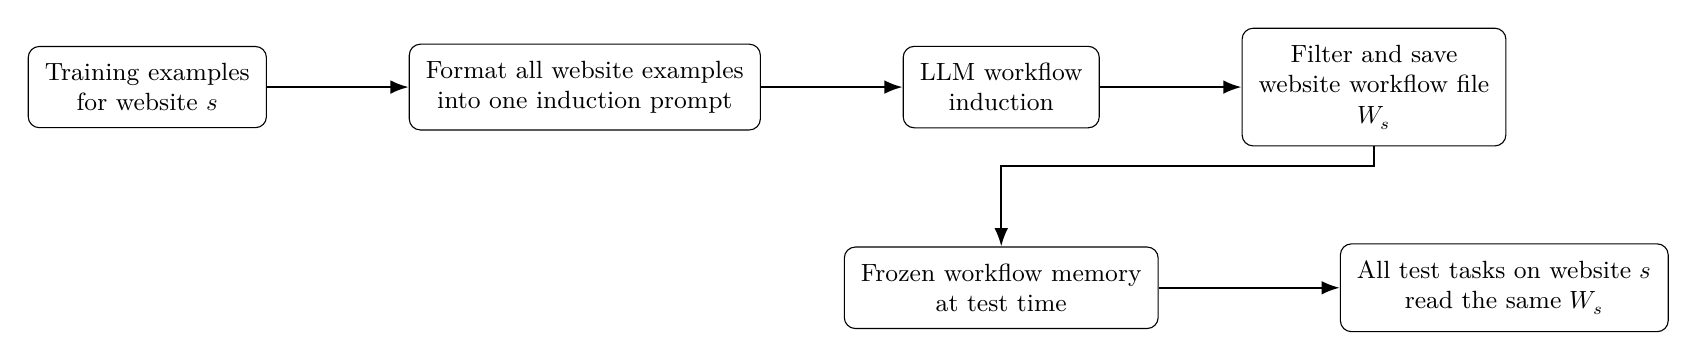
\begin{tikzpicture}[
  >=Latex,
  node distance=1.3cm and 1.8cm,
  box/.style={draw, rounded corners, align=center, inner sep=6pt, font=\small},
  flow/.style={->, thick}
]

\node[box] (train) {Training examples\\for website \(s\)};
\node[box, right=of train] (prompt) {Format all website examples\\into one induction prompt};
\node[box, right=of prompt] (llm) {LLM workflow\\induction};
\node[box, right=of llm] (save) {Filter and save\\website workflow file\\\(W_s\)};
\node[box, below=1.5cm of llm] (frozen) {Frozen workflow memory\\at test time};
\node[box, right=2.3cm of frozen] (test) {All test tasks on website \(s\)\\read the same \(W_s\)};

\draw[flow] (train) -- (prompt);
\draw[flow] (prompt) -- (llm);
\draw[flow] (llm) -- (save);
\draw[flow] (save) -- ++(0.0,-1.0) -| (frozen.north);
\draw[flow] (frozen) -- (test);

\end{tikzpicture}%
}
\caption{Website-level operationalization of offline induction in the current Mind2Web reproduction.}
\label{fig:offline-induction-one-shot}
\end{figure}

Crucially, the current offline pipeline induces workflows once from all
available training examples of a website, saves a single
website-specific workflow file \(W_s\), and then keeps that file fixed
during test-time inference. Unlike the online setting, there is no
prefix update loop: all test tasks on the same website receive the same
frozen workflow memory.

\subsection{Online Induction}\label{online-induction}

Without training examples, AWM operates in online mode. The agent
processes test queries sequentially; after each task, an LM-based
evaluator judges success. Successful trajectories are used to induce new
workflows, which accumulate in memory for subsequent tasks. This creates
a snowball effect: later tasks benefit from workflows induced from
earlier successes. The paper presents this as especially useful under
larger distribution shift because the workflows are derived from
test-time rather than training-time experience.

The paper distinguishes Mind2Web and WebArena at the level of benchmark
setup and evaluation protocol, but it does not present two different
online-induction mechanisms for the two benchmarks. At the method level,
online AWM is described uniformly as a success-gated process: the agent
first solves a test task, an evaluator then judges whether the resulting
experience is successful, and only successful experiences are
transformed into workflows and added to memory. However, the released
implementations do not instantiate this mechanism identically across
benchmarks. The WebArena pipeline remains broadly consistent with the
paper-level description by filtering trajectories through a reward or
auto-evaluation success criterion before induction, whereas the
Mind2Web implementation re-induces workflows from all available prefix
result JSONs without an explicit success-only filter. Therefore, in this
reproduction, the paper-level online-AWM description and the
benchmark-specific implementation details must be distinguished
carefully, especially when interpreting mechanism claims from Mind2Web
runs. This discrepancy is recorded as a benchmark-specific
implementation note in the released code path; this study follows the
released Mind2Web pipeline as-is, and the note is not treated here as
a methodological objection to AWM in general.

\paragraph{Operational flow in the current reproduction pipeline.}
The current Mind2Web reproduction instantiates online induction as a
prefix-level overwrite loop:

\begin{figure}[htbp]
\centering
\resizebox{0.92\linewidth}{!}{%
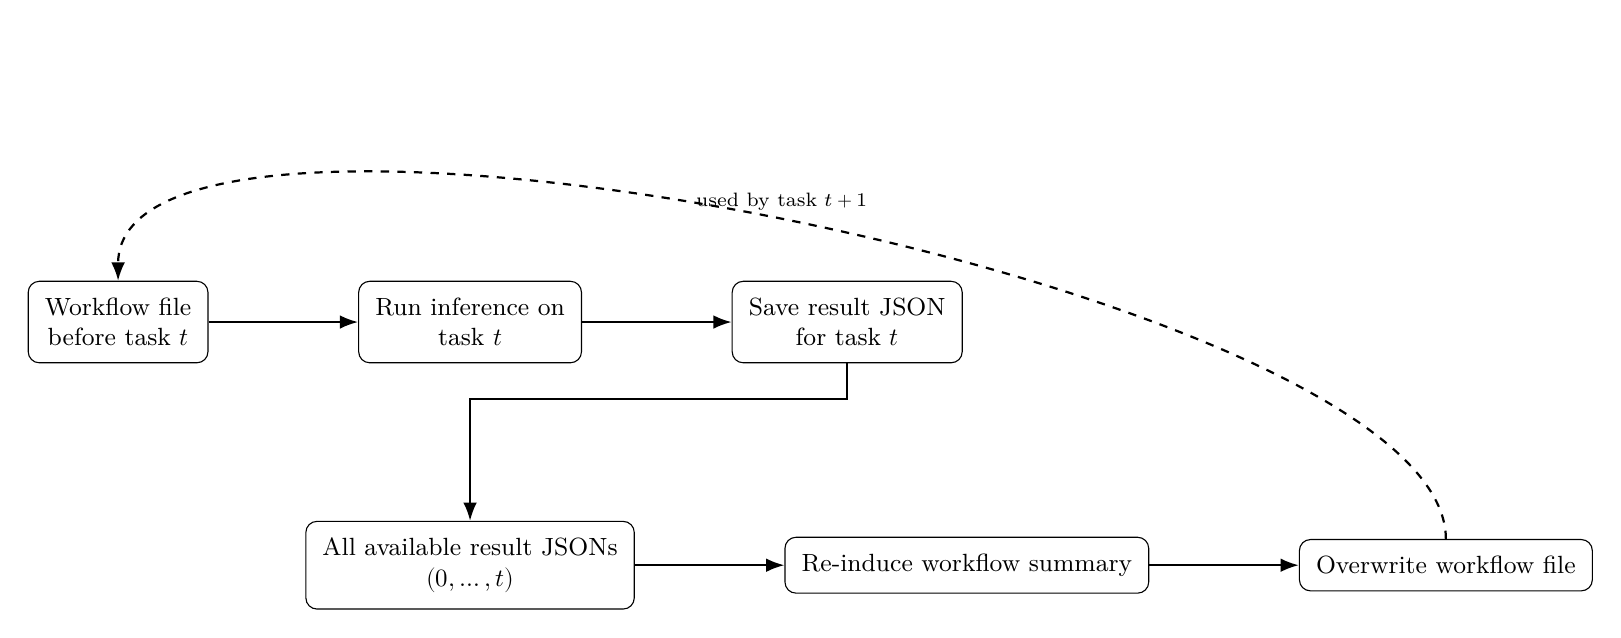
\begin{tikzpicture}[
  >=Latex,
  node distance=1.5cm and 1.9cm,
  box/.style={draw, rounded corners, align=center, inner sep=6pt, font=\small},
  flow/.style={->, thick},
  loopflow/.style={->, dashed, thick}
]

\node[box] (wf) {Workflow file\\before task \(t\)};
\node[box, right=of wf] (infer) {Run inference on\\task \(t\)};
\node[box, right=of infer] (json) {Save result JSON\\for task \(t\)};

\node[box, below=2.0cm of infer] (prefix) {All available result JSONs\\\((0,\dots,t)\)};
\node[box, right=of prefix] (induce) {Re-induce workflow summary};
\node[box, right=of induce] (overwrite) {Overwrite workflow file};

\draw[flow] (wf) -- (infer);
\draw[flow] (infer) -- (json);

\draw[flow] (json.south) -- ++(0,-0.45) -| ([xshift=0pt]prefix.north);
\draw[flow] (prefix) -- (induce);
\draw[flow] (induce) -- (overwrite);

\draw[loopflow] (overwrite.north) .. controls +(0,3.2) and +(0,3.2) .. node[above, font=\scriptsize] {used by task \(t+1\)} (wf.north);

\end{tikzpicture}%
}
\caption{Prefix-level operationalization of online induction in the current Mind2Web reproduction.}
\label{fig:online-induction-prefix-loop}
\end{figure}

Crucially, task \(t\) is solved using workflow memory induced from
earlier tasks only, not from its own trajectory. After task \(t\) is
completed, its result JSON is added to the available prefix result set,
and the workflow file is re-induced from the full prefix
\((0,\dots,t)\). Under \texttt{induce\_steps = 1}, task \(2\) is
therefore evaluated using a workflow file re-induced from the completed
result JSONs of tasks \(0\) and \(1\). The update is overwrite-based
over the full available prefix, rather than an append-only ``old
workflow + newest trajectory'' merge.
If \(t\) is the final task in the stream, the pipeline stops after
saving its result JSON and no further induction round is triggered.
Moreover, the induction module does not directly read the previous
workflow file: its direct input is the available prefix result JSONs
only. Any influence from earlier workflow memory can persist only
indirectly, because some later result JSONs may already reflect
workflow-conditioned behavior from earlier tasks.

\subsection{Rule-Induction
Baseline}\label{rule-induction-baseline}

As an ablation, the paper proposes rule-based induction, which extracts
each unique experience's action sequence directly without abstraction.
This produces complete concrete trajectory copies rather than
parameterized sub-routines, serving as a comparison point for isolating
the contribution of LM-based abstraction.

\subsection{Mind2Web Evaluation
Protocol}\label{mind2web-evaluation-protocol}

On Mind2Web, each task has a fixed number of steps. Per-step evaluation
measures:

\begin{itemize}
\tightlist
\item
  \textbf{Element Accuracy} --- whether the correct page element is
  selected
\item
  \textbf{Action F1} --- whether the action on that element is correct
\item
  \textbf{Step Success Rate (SR)} --- whether both element and action
  are correct
\item
  \textbf{Task Success Rate} --- whether all steps in a task succeed
\end{itemize}

The benchmark provides three evaluation splits: \textbf{cross-task}
(same website, different tasks), \textbf{cross-website} (same domain,
different website), and \textbf{cross-domain} (different domain
entirely).

To align the system description with the course requirement on system
modeling and structure, Table~\ref{tab:awm-design-choice-rationale}
summarizes the AWM design choices that matter most in this reproduction,
the limitations they are meant to address, and the later sections where
those design claims are audited.

{\begin{longtable}[]{@{}
  >{\raggedright\arraybackslash}p{(\linewidth - 4\tabcolsep) * \real{0.30}}
  >{\raggedright\arraybackslash}p{(\linewidth - 4\tabcolsep) * \real{0.34}}
  >{\raggedright\arraybackslash}p{(\linewidth - 4\tabcolsep) * \real{0.36}}@{}}
\caption{AWM design choices, the limitations they target, and where this study audits them.}\label{tab:awm-design-choice-rationale}\\

\toprule\noalign{}
\begin{minipage}[b]{\linewidth}\raggedright
AWM Design Choice
\end{minipage} & \begin{minipage}[b]{\linewidth}\raggedright
Existing Limitation It Addresses
\end{minipage} & \begin{minipage}[b]{\linewidth}\raggedright
Where This Study Audits It
\end{minipage} \\
\midrule\noalign{}
\endhead
\bottomrule\noalign{}
\endlastfoot
Parameterized workflows with placeholders (§3.2) & Raw trajectory replay
does not generalize well across tasks with different values and surface
forms & §5.4 and Section~\ref{mechanism-audit}, especially the
value-guidance case analysis \\
Offline induction with frozen test-time memory (§3.3) & When annotated
data is available, repeated online rewriting introduces avoidable noise
and extra compute & §5.2 and Section~\ref{offline-vs-online-trade-off} \\
Online incremental induction in the paper-level design (§3.4) &
Annotated training examples may be unavailable, so memory must grow from
test-time experience & §5.3, Section~\ref{small-data-efficiency}, and
Section~\ref{threats-to-validity} \\
Rule-induction baseline (§3.5) & The contribution of LM-based
abstraction cannot be isolated without a non-abstract trajectory-memory
counterpart & §5.4 \\
Text-only workflow memory via prompt injection (§3.2) & Executable skill
libraries require heavier infrastructure than many web-agent pipelines
can support & §5.5 and Section~\ref{mechanism-audit} \\
\end{longtable}
}

Design-level refinements proposed by this study to address the audited
failure modes are collected in
Section~\ref{design-implications-and-proposed-refinements}.

\section{Experimental Setup and Analysis Protocol}\label{reproduction-methodology}

\subsection{Evaluated Claims}\label{claim-structure}

We evaluate five groups of claims from the Mind2Web portion of the
paper:

{\begin{longtable}[]{@{}
  >{\raggedright\arraybackslash}p{(\linewidth - 4\tabcolsep) * \real{0.1395}}
  >{\raggedright\arraybackslash}p{(\linewidth - 4\tabcolsep) * \real{0.3023}}
  >{\raggedright\arraybackslash}p{(\linewidth - 4\tabcolsep) * \real{0.5581}}@{}}
\toprule\noalign{}
\begin{minipage}[b]{\linewidth}\raggedright
Setting
\end{minipage} & \begin{minipage}[b]{\linewidth}\raggedright
Paper Claim
\end{minipage} & \begin{minipage}[b]{\linewidth}\raggedright
Evaluation in This Study
\end{minipage} \\
\midrule\noalign{}
\endhead
\bottomrule\noalign{}
\endlastfoot
\textbf{Offline cross-task memory} & Offline AWM improves cross-task Step SR & Offline workflow
vs.~no-workflow on 7 websites \\
\textbf{Online cross-site generalization} & Online AWM generalizes under larger distribution gap &
Online workflow on cross-task (kayak), cross-website (tripadvisor),
cross-domain (reddit) \\
\textbf{LM vs.~rule induction} & LM induction outperforms rule induction & LM vs.~rule
workflow on 3 websites (newegg, united, kayak) \\
\shortstack[l]{\textbf{Representation}\\\textbf{ablations}} & Code/text difference is small;\newline NL \textgreater{} HTML observation & Code/text on kayak; NL/HTML on 3 websites \\
\textbf{Workflow quality} & Compact workflow libraries with high utility and low
overlap & Workflow text analysis on 3 websites \\
\end{longtable}
}

\subsection{Models and Data}\label{models-and-data}

The experiments use \textbf{GPT-4o} and \textbf{Qwen-3.5-397B-A17B}
(referred to as Qwen throughout) on Mind2Web. The evaluated sites
include kayak, newegg, united, budget, sixflags, yellowpages, and
kohls, plus cross-site targets Tripadvisor and Reddit for the online
generalization setting.

\subsection{Analysis Methods}\label{analysis-methods}

To go beyond aggregate score comparison, we use four complementary
analysis tools.

\paragraph{4.3.1 Step-Level
Decomposition}\label{step-level-decomposition}

We decomposed the workflow-minus-baseline delta along three dimensions:

\begin{itemize}
\tightlist
\item
  \textbf{By action type} (CLICK / TYPE / SELECT): isolates whether
  gains come from element grounding or action/value guidance.
\item
  \textbf{By step position} (first half / second half): tests whether
  workflow helps at task initiation or throughout the trajectory.
\item
  \textbf{By website}: contrasts reproduced vs.~not-reproduced sites.
\end{itemize}

\paragraph{4.3.2 Paired-Case Analysis}\label{paired-case-analysis}

For each step in each task, we classified the baseline--workflow pair
into four categories:

{\begin{longtable}[]{@{}llll@{}}
\toprule\noalign{}
Category & Baseline & +Workflow & Interpretation \\
\midrule\noalign{}
\endhead
\bottomrule\noalign{}
\endlastfoot
\textbf{Positive} & 0 & 1 & Workflow genuinely helped \\
\textbf{Negative} & 1 & 0 & Workflow caused harm \\
\textbf{Ineffective} & 0 & 0 & Workflow made no difference \\
\textbf{Redundant} & 1 & 1 & Workflow was unnecessary \\
\end{longtable}
}

This produces a distribution that reveals how many steps are actually
affected by workflow injection and whether the net effect is positive or
negative.

\paragraph{4.3.3 Prompt-Level Case Study}\label{prompt-level-case-study}

Selected paired cases are traced back to raw JSON prompts and action
outputs. This allows mechanism interpretation at the case level: whether
the output change is causally attributable to a specific workflow
instruction.

\paragraph{4.3.4 Auxiliary Analyses}\label{auxiliary-analyses}

We additionally use target-site result tracing in the online
generalization setting, workflow-text comparison, an
exploratory alignment heuristic, a direct offline-vs.-online
comparison, and prefix-level online learning curves to sharpen the main
reproduction findings.

\section{Reproduction Results}\label{reproduction-results}

\subsection{Main Reproduction
Findings}\label{overall-reproduction-status}

{\begin{longtable}[]{@{}
  >{\raggedright\arraybackslash}p{(\linewidth - 4\tabcolsep) * \real{0.2188}}
  >{\raggedright\arraybackslash}p{(\linewidth - 4\tabcolsep) * \real{0.2500}}
  >{\raggedright\arraybackslash}p{(\linewidth - 4\tabcolsep) * \real{0.5312}}@{}}
\caption{Summary of main reproduction findings.}\label{tab:summary-of-main-reproduction-findings}\\

\toprule\noalign{}
\begin{minipage}[b]{\linewidth}\raggedright
Claim
\end{minipage} & \begin{minipage}[b]{\linewidth}\raggedright
Evidence Base
\end{minipage} & \begin{minipage}[b]{\linewidth}\raggedright
Main Finding
\end{minipage} \\
\midrule\noalign{}
\endhead
\bottomrule\noalign{}
\endlastfoot
\textbf{Offline cross-task memory}: Offline AWM improves cross-task Step SR & Mind2Web first run &
Mixed; positive on 2/7 sites, negative on 2/7 sites, and mixed on 3/7
sites \\
\textbf{Online cross-site generalization}: Online AWM generalizes under larger gap & Mind2Web first run &
Overall direction unsupported \\
\textbf{LM vs.~rule induction}: LM induction outperforms rule induction & Mind2Web first run &
Text-level difference strongly supported; performance
advantage mixed \\
\textbf{Representation ablations}: Code/text similar; NL \textgreater{} HTML & Mind2Web first run &
Code/text supported on kayak; NL \textgreater{} HTML not
supported after a three-site evaluation \\
\textbf{Workflow quality}: Compact, high-utility, low-overlap library & Mind2Web first run &
Supported under prompt-level proxy; utility proxy remains
loose \\
\end{longtable}
}

This already reveals an asymmetry: the paper's \textbf{mechanistic and
structural} claims hold up better than its strongest \textbf{performance
and generalization} claims.

\subsection{Offline AWM on Cross-Task
Generalization}\label{c1-offline-awm-on-cross-task-generalization}

The offline story is mixed rather than uniformly positive. Some sites
benefit, some degrade, and some remain genuinely mixed.

\paragraph{5.2.1 Step-Level Decomposition by Action
Type}\label{step-level-decomposition-by-action-type}

{\begin{longtable}[]{@{}
  >{\raggedright\arraybackslash}p{(\linewidth - 10\tabcolsep) * \real{0.1875}}
  >{\raggedright\arraybackslash}p{(\linewidth - 10\tabcolsep) * \real{0.2292}}
  >{\raggedleft\arraybackslash}p{(\linewidth - 10\tabcolsep) * \real{0.1458}}
  >{\raggedleft\arraybackslash}p{(\linewidth - 10\tabcolsep) * \real{0.1458}}
  >{\raggedleft\arraybackslash}p{(\linewidth - 10\tabcolsep) * \real{0.1458}}
  >{\raggedleft\arraybackslash}p{(\linewidth - 10\tabcolsep) * \real{0.1458}}@{}}
\caption{Step-level delta by action type (offline\_wf - no\_workflow, GPT-4o, cross-task).}\label{tab:step-level-delta-by-action-type-offline-wf-no}\\

\toprule\noalign{}
\begin{minipage}[b]{\linewidth}\raggedright
Website
\end{minipage} & \begin{minipage}[b]{\linewidth}\raggedright
Outcome
\end{minipage} & \begin{minipage}[b]{\linewidth}\raggedleft
CLICK \ensuremath{\Delta}Elem
\end{minipage} & \begin{minipage}[b]{\linewidth}\raggedleft
CLICK \ensuremath{\Delta}SR
\end{minipage} & \begin{minipage}[b]{\linewidth}\raggedleft
TYPE \ensuremath{\Delta}ActF1
\end{minipage} & \begin{minipage}[b]{\linewidth}\raggedleft
TYPE \ensuremath{\Delta}SR
\end{minipage} \\
\midrule\noalign{}
\endhead
\bottomrule\noalign{}
\endlastfoot
kayak & positive & +10.7\% & +10.7\% & +1.4\% & +0.0\% \\
newegg & positive & +9.1\% & +6.1\% & +50.0\% & +33.3\% \\
united & mixed & +0.0\% & +0.0\% & +19.5\% & +28.6\% \\
budget & negative & \textbf{-12.1\%} & \textbf{-12.1\%} & +8.4\% &
+9.1\% \\
sixflags & negative & \textbf{-6.1\%} & \textbf{-6.1\%} & +0.0\% &
+0.0\% \\
\end{longtable}
}

\textbf{TYPE-side value guidance is the most stable positive effect.}
Even on negative-outcome sites, TYPE Action F1 improves (budget +8.4\%).
Workflows provide value templates --- city names, search keywords, price
ranges --- that help the model choose correct input values regardless of
site match quality.

\textbf{CLICK-side grounding is the main source of divergence across
sites.} Positive-outcome sites show +9--11\% CLICK Element
Accuracy gains; negative-outcome sites show -6 to -12\% degradation.
Workflow-provided element descriptions help when they match the target
HTML structure and actively mislead when they do not. CLICK performance
is the primary factor separating positive and negative outcomes.
Appendix~\ref{app:A1} provides the underlying step-level summary behind
these action-type claims.

\paragraph{5.2.2 Step-Level Decomposition by Trajectory
Position}\label{step-level-decomposition-by-trajectory-position}

{\begin{longtable}[]{@{}llrr@{}}
\caption{Step SR delta by trajectory half (offline\_wf - no\_workflow, GPT-4o, cross-task).}\label{tab:step-sr-delta-by-trajectory-half-offline-wf-n}\\

\toprule\noalign{}
Website & Outcome & First Half \ensuremath{\Delta}SR & Second Half \ensuremath{\Delta}SR \\
\midrule\noalign{}
\endhead
\bottomrule\noalign{}
\endlastfoot
kayak & positive & +0.0\% & \textbf{+13.0\%} \\
newegg & positive & +4.4\% & +7.1\% \\
budget & negative & -1.9\% & \textbf{-10.9\%} \\
sixflags & negative & -5.9\% & -3.3\% \\
\end{longtable}
}

Workflow effects accumulate over the trajectory. On kayak, the entire
gain comes from the second half (+13\% vs.~+0\%). On budget, degradation
worsens in the second half (-10.9\% vs.~-1.9\%). AWM is not merely a
``first-step hint'' --- its influence grows as the trajectory lengthens,
amplifying either help or harm.

\paragraph{5.2.3 Paired-Case
Distribution}\label{paired-case-distribution}

{\begin{longtable}[]{@{}
  >{\raggedright\arraybackslash}p{(\linewidth - 12\tabcolsep) * \real{0.1636}}
  >{\raggedright\arraybackslash}p{(\linewidth - 12\tabcolsep) * \real{0.2000}}
  >{\raggedleft\arraybackslash}p{(\linewidth - 12\tabcolsep) * \real{0.1273}}
  >{\raggedleft\arraybackslash}p{(\linewidth - 12\tabcolsep) * \real{0.1273}}
  >{\raggedleft\arraybackslash}p{(\linewidth - 12\tabcolsep) * \real{0.1273}}
  >{\raggedleft\arraybackslash}p{(\linewidth - 12\tabcolsep) * \real{0.1273}}
  >{\raggedleft\arraybackslash}p{(\linewidth - 12\tabcolsep) * \real{0.1273}}@{}}
\caption{Paired-case distribution (GPT-4o, cross-task, 475 paired steps across 7 sites).}\label{tab:paired-case-distribution-gpt-4o-cross-task-47}\\

\toprule\noalign{}
\begin{minipage}[b]{\linewidth}\raggedright
Website
\end{minipage} & \begin{minipage}[b]{\linewidth}\raggedright
Outcome
\end{minipage} & \begin{minipage}[b]{\linewidth}\raggedleft
Positive
\end{minipage} & \begin{minipage}[b]{\linewidth}\raggedleft
Negative
\end{minipage} & \begin{minipage}[b]{\linewidth}\raggedleft
Ineffective
\end{minipage} & \begin{minipage}[b]{\linewidth}\raggedleft
Redundant
\end{minipage} & \begin{minipage}[b]{\linewidth}\raggedleft
Net
\end{minipage} \\
\midrule\noalign{}
\endhead
\bottomrule\noalign{}
\endlastfoot
kayak & positive & 3 & \textbf{0} & 22 & 23 & +3 \\
newegg & positive & 5 & \textbf{0} & 56 & 26 & +5 \\
united & mixed & 3 & 2 & 35 & 23 & +1 \\
budget & negative & 6 & \textbf{12} & 53 & 28 & -6 \\
sixflags & negative & 3 & \textbf{6} & 23 & 32 & -3 \\
\end{longtable}
}

Three patterns emerge:

\begin{enumerate}
\def\labelenumi{\arabic{enumi}.}
\item
  \textbf{On positive-outcome sites, workflow never harms the agent} (negative
  = 0). AWM either helps or does nothing, but never misleads. This ``do
  no harm'' property is the key precondition for AWM to work.
\item
  \textbf{On negative-outcome sites, negative interventions substantially
  outnumber positive ones.} Budget shows 12 negative vs.~6 positive;
  sixflags shows 6 vs.~3. When the workflow does not match the target
  site, it becomes a net source of harm.
\item
  \textbf{AWM's actual influence window is narrow.} Ineffective steps
  constitute 45--65\% of all steps. Workflow genuinely changes model
  behavior on only 6--18\% of steps. The aggregate Step SR improvement
  is driven by a small number of decisive interventions, not by uniform
  all-step guidance.
\end{enumerate}

Appendix~\ref{app:A2} records the corrected 475-step paired-case totals
used in this subsection.

\subsection{Online AWM Under Larger Distribution
Shift}\label{c2-online-awm-under-larger-distribution-shift}

This is the clearest challenge to the paper's global narrative.

\paragraph{5.3.1 Cross-Site Results}\label{cross-site-results}

{\begin{longtable}[]{@{}lrrrr@{}}
\caption{Online workflow paired-case results on cross-site targets (Qwen).}\\

\toprule\noalign{}
Target Site & Positive & Negative & Net & Pos/(Pos+Neg) \\
\midrule\noalign{}
\endhead
\bottomrule\noalign{}
\endlastfoot
tripadvisor & 4 & \textbf{18} & \textbf{-14} & 18.2\% \\
reddit & 2 & \textbf{5} & \textbf{-3} & 28.6\% \\
\end{longtable}
\label{tab:online-workflow-paired-case-results-on-cross-site-qwen-main}
}

The paper claims that ``online AWM shows larger advantage under larger
distribution gap.'' Our first-run results show the opposite: online
workflows produce net negative outcomes on both target sites, with
tripadvisor suffering particularly severe degradation.

\paragraph{5.3.2 First-Run Target-Site Result
Tracing}\label{cross-site-degradation-diagnosis}

To characterize what happened on the two available target sites, we use
two descriptive checks:

\begin{itemize}
\tightlist
\item
  \textbf{Check A (prompt/action mismatch pattern):} Are the negative
  steps dominated by early action-pattern errors such as wrong
  `CLICK`/`TYPE` choices?
\item
  \textbf{Check B (baseline candidate quality):} Does the target site's
  baseline show a much higher `skip rate`, suggesting weaker candidate
  quality?
\end{itemize}

{\begin{longtable}[]{@{}
  >{\raggedright\arraybackslash}p{(\linewidth - 4\tabcolsep) * \real{0.3095}}
  >{\raggedright\arraybackslash}p{(\linewidth - 4\tabcolsep) * \real{0.4524}}
  >{\raggedright\arraybackslash}p{(\linewidth - 4\tabcolsep) * \real{0.2381}}@{}}
\caption{First-run target-site result tracing.}\label{tab:cross-site-degradation-diagnosis}\\

\toprule\noalign{}
\begin{minipage}[b]{\linewidth}\raggedright
Target Site
\end{minipage} & \begin{minipage}[b]{\linewidth}\raggedright
Descriptive Reading
\end{minipage} & \begin{minipage}[b]{\linewidth}\raggedright
Key Evidence
\end{minipage} \\
\midrule\noalign{}
\endhead
\bottomrule\noalign{}
\endlastfoot
tripadvisor & first-run underperformance with weaker baseline candidate
quality & Skip rate +16pp; 14/18 negatives are CLICK \\
reddit & first-run underperformance without obvious baseline collapse &
Skip rate only +4.7pp; baseline CLICK EA higher than source; 4/5 negatives are CLICK \\
\end{longtable}
}

\textbf{The safest reading is a result-level one.} In the current
first run, online workflows underperform baseline on both target sites.
On tripadvisor, the result trace also shows weaker baseline candidate
quality. Appendix~\ref{app:A3} summarizes these first-run facts, and
Appendix~\ref{app:B6} provides a manually verified prompt-level case in
which workflow memory is already present when the wrong first action is
produced. These materials should be read as result tracing and
case-level evidence, not as standalone causal proof.

\subsection{LM-Induced vs Rule-Induced
Workflows}\label{c3-lm-induced-vs-rule-induced-workflows}

This is the strongest explanatory finding in the study.

\paragraph{5.4.1 Text-Level Differences}\label{text-level-differences}

{\begin{longtable}[]{@{}
  >{\raggedright\arraybackslash}p{(\linewidth - 12\tabcolsep) * \real{0.1765}}
  >{\raggedleft\arraybackslash}p{(\linewidth - 12\tabcolsep) * \real{0.1373}}
  >{\raggedleft\arraybackslash}p{(\linewidth - 12\tabcolsep) * \real{0.1373}}
  >{\raggedleft\arraybackslash}p{(\linewidth - 12\tabcolsep) * \real{0.1373}}
  >{\raggedleft\arraybackslash}p{(\linewidth - 12\tabcolsep) * \real{0.1373}}
  >{\raggedleft\arraybackslash}p{(\linewidth - 12\tabcolsep) * \real{0.1373}}
  >{\raggedleft\arraybackslash}p{(\linewidth - 12\tabcolsep) * \real{0.1373}}@{}}
\caption{Workflow text features: LM vs.~rule induction.}\label{tab:workflow-text-features-lm-vs-rule-induction}\\

\toprule\noalign{}
\begin{minipage}[b]{\linewidth}\raggedright
Feature
\end{minipage} & \begin{minipage}[b]{\linewidth}\raggedleft
kayak LM
\end{minipage} & \begin{minipage}[b]{\linewidth}\raggedleft
kayak Rule
\end{minipage} & \begin{minipage}[b]{\linewidth}\raggedleft
newegg LM
\end{minipage} & \begin{minipage}[b]{\linewidth}\raggedleft
newegg Rule
\end{minipage} & \begin{minipage}[b]{\linewidth}\raggedleft
united LM
\end{minipage} & \begin{minipage}[b]{\linewidth}\raggedleft
united Rule
\end{minipage} \\
\midrule\noalign{}
\endhead
\bottomrule\noalign{}
\endlastfoot
Workflow count & 8 & 17 & 6 & 19 & 6 & 24 \\
Total steps & 14 & 213 & 10 & 149 & 16 & 217 \\
Avg steps/WF & \textbf{1.8} & 12.5 & \textbf{1.7} & 7.8 & \textbf{2.7} &
9.0 \\
Placeholders & \textbf{13} & 0 & \textbf{6} & 0 & \textbf{15} & 0 \\
Concrete values & 0 & \textbf{25} & 0 & \textbf{16} & 0 & \textbf{41} \\
\end{longtable}
}

LM-induced workflows are consistently more abstract at the text level:
fewer (6--8 vs.~17--24), shorter (1.7--2.7 vs.~7.8--12.5 steps/WF),
fully parameterized, and contain zero concrete values. All four
text-level indicators confirm the paper's abstraction narrative on all
three sites (see Appendices~\ref{app:C1}, \ref{app:C2}, and
\ref{app:C3}).

\paragraph{5.4.2 Performance-Level
Qualification}\label{performance-level-qualification}

However, textual abstraction does not automatically translate to
performance superiority.

{\begin{longtable}[]{@{}lrrl@{}}
\caption{LM vs.~rule net paired gains (Qwen, cross-task).}\label{tab:lm-vs-rule-net-paired-gains-qwen-cross-task}\\

\toprule\noalign{}
Website & LM Net Gain & Rule Net Gain & Direction \\
\midrule\noalign{}
\endhead
\bottomrule\noalign{}
\endlastfoot
newegg & +2 & +4 & Rule ≥ LM \\
united & +1 & -2 & LM \textgreater{} Rule \\
kayak & 0 & -1 & LM ≥ Rule \\
\end{longtable}
}

On newegg, where cross-task operational patterns are relatively fixed
(search → filter → sort → cart), rule workflows' concrete values happen
to match the test tasks well. For newegg, the evidence therefore remains
mixed. On united, where task diversity is higher, LM's
abstraction provides clearer benefit. The paper reports only the
aggregate LM \textgreater{} Rule conclusion without discussing this
boundary condition.

\subsection{Representation
Ablations}\label{c4-representation-ablations}

\paragraph{5.5.1 Code vs Text Workflow}\label{code-vs-text-workflow}

On kayak (Qwen), code and text workflows perform similarly (Step SR
difference: 2.2pp), consistent with the paper's claim that format itself
is not the decisive factor. However, both perform below the no-workflow
baseline (51.2\%), so the stronger implied reading that both formats are
reliably beneficial is only directionally supported.

\paragraph{5.5.2 NL vs HTML Observation}\label{nl-vs-html-observation}

{\begin{longtable}[]{@{}lrrrl@{}}
\caption{Step SR by observation representation (Qwen, three sites).}\label{tab:step-sr-by-observation-representation-qwen-th}\\

\toprule\noalign{}
Site & desc\_only & html\_only & desc\_html & Paper Prediction \\
\midrule\noalign{}
\endhead
\bottomrule\noalign{}
\endlastfoot
kayak & 45.3 & 48.0 & 50.3 & NOT supported \\
newegg & \textbf{30.5} & 23.9 & 30.3 & Supported \\
united & 55.9 & \textbf{60.6} & 51.7 & NOT supported \\
\end{longtable}
}

The paper's claim that NL descriptions are generally superior to HTML is
not supported in the three-site evaluation. Only NewEgg supports it. On
United, html\_only is best --- likely because United's HTML element
names are inherently readable (e.g., \texttt{tab\ TRAVEL\ INFO},
\texttt{heading\ Check-in}). The mixed representation (desc\_html)
causes the most severe degradation on united: task SR drops from 33.3\%
to 16.7\%, consistent with attention dilution from increased prompt
length and redundancy.

\textbf{The broader takeaway is that representation preference is
site-dependent, not globally uniform.} Appendix~\ref{app:A4} collects
the first-run result table behind this subsection.

\subsection{Workflow Quality}\label{c5-workflow-quality}

Under current proxy definitions, the paper's workflow-quality story is
broadly supported: workflow libraries are compact (5--7 LM workflows per
site), overlap is low (0--3.33\%), and prompt-level utility is high
(100\% injection rate).

But this must be reported carefully. Prompt-level utility is not the
same as behavior-level adherence. When paired-case evidence is taken
into account, AWM's actual causal reach is much sparser than a naive
reading of ``high utility'' would suggest. The gap between ``workflow is
present in the prompt'' and ``workflow changes the model's behavior'' is
large: only 6--18\% of steps show actual behavioral change.
Appendix~\ref{app:A5} gives the workflow-quality table and its proxy
limitations.

\section{Mechanistic Analysis}\label{mechanism-audit}

The analysis in this section is a first-run interpretive reading
grounded in the step-level decomposition, the paired-case distribution,
and the manually verified prompt-level case studies. The positive and
negative mechanisms described below are consistent with the audited
evidence on the covered sites, but single-run data cannot rule out
run-to-run variation. Repeated trials with variance estimation would be
required before these readings are treated as causally identified
mechanism claims.

\subsection{Where the Gains Come
From}\label{where-the-gains-come-from}

The most stable gain channel is \textbf{TYPE-side value guidance}.
Workflows help the model supply the correct kind of parameter, value
format, or label target. This channel remains positive even on sites
where AWM is overall harmful.

The more fragile channel is \textbf{CLICK-side grounding}. This channel
works only when workflow language matches the site's operational
structure. On a matched site, it is helpful; on a mismatched site, it
becomes a source of false anchoring.

\subsection{Sparse Intervention Rather Than Uniform
Guidance}\label{sparse-intervention-rather-than-uniform-guidance}

The paired-case analysis shows that workflow is not exerting continuous
control. Most steps are ineffective or redundant. AWM should not be
understood as ``guiding the entire trajectory.'' It is better understood
as a \textbf{sparse intervention mechanism} that occasionally changes
high-leverage decisions.

\subsection{Prompt-Level Positive
Mechanisms}\label{prompt-level-positive-mechanisms}

Six manually verified case studies (three positive, three negative) were
traced back to raw JSON prompts. All six have been confirmed against the
original data files. Representative positive cases are shown in
Appendices~\ref{app:B1} and \ref{app:B2}.

\paragraph{P-1: Preventing Premature Termination (kayak, task 1, step
9)}\label{p-1-preventing-premature-termination-kayak-task-1-step-9}

\textbf{Task:} ``Find the cheapest Hawaii package for two adults from
June 18 to 21''

{\begin{longtable}[]{@{}
  >{\raggedright\arraybackslash}p{(\linewidth - 4\tabcolsep) * \real{0.3333}}
  >{\raggedright\arraybackslash}p{(\linewidth - 4\tabcolsep) * \real{0.3333}}
  >{\raggedright\arraybackslash}p{(\linewidth - 4\tabcolsep) * \real{0.3333}}@{}}
\toprule\noalign{}
\begin{minipage}[b]{\linewidth}\raggedright
\end{minipage} & \begin{minipage}[b]{\linewidth}\raggedright
Baseline
\end{minipage} & \begin{minipage}[b]{\linewidth}\raggedright
Workflow
\end{minipage} \\
\midrule\noalign{}
\endhead
\bottomrule\noalign{}
\endlastfoot
step\_success & 0 & \textbf{1} \\
Model output & Empty pred\_act; outputs natural language summary about
car rental (hallucination) & \texttt{CLICK\ {[}57318{]}} (Sort by
Cheapest) \\
Failure mode & Model hallucinates task completion, outputs ungrounded
text & --- \\
\end{longtable}
}

\textbf{Mechanism:} Workflow 8 (\texttt{View\ and\ Select\ Deals})
prompts ``HOVER/CLICK to view deals on the results page,'' preventing
premature termination.

\paragraph{P-2: Strategy Redirection (newegg, task 4, step
0)}\label{p-2-strategy-redirection-newegg-task-4-step-0}

\textbf{Task:} ``Find a new drone priced between 25 to 50 dollar and
ships from USA\ldots{}''

{\begin{longtable}[]{@{}
  >{\raggedright\arraybackslash}p{(\linewidth - 4\tabcolsep) * \real{0.3333}}
  >{\raggedright\arraybackslash}p{(\linewidth - 4\tabcolsep) * \real{0.3333}}
  >{\raggedright\arraybackslash}p{(\linewidth - 4\tabcolsep) * \real{0.3333}}@{}}
\toprule\noalign{}
\begin{minipage}[b]{\linewidth}\raggedright
\end{minipage} & \begin{minipage}[b]{\linewidth}\raggedright
Baseline
\end{minipage} & \begin{minipage}[b]{\linewidth}\raggedright
Workflow
\end{minipage} \\
\midrule\noalign{}
\endhead
\bottomrule\noalign{}
\endlastfoot
step\_success & 0 & \textbf{1} \\
Model output & \texttt{CLICK\ {[}10463{]}} (Electronics category
navigation) & \texttt{TYPE\ {[}126{]}\ {[}drone{]}} (search box) \\
Failure mode & Defaults to ``browse categories'' strategy & --- \\
\end{longtable}
}

\textbf{Mechanism:} \texttt{search\_and\_apply\_filters} workflow's
first step is
\texttt{{[}searchbox{]}\ Search\ Site\ →\ TYPE:\ \{search-term\}},
redirecting from ``browse-first'' to ``search-first'' strategy.

\paragraph{P-3: Value Format Correction (newegg, task 5, step
3)}\label{p-3-value-format-correction-newegg-task-5-step-3}

\textbf{Task:} ``Find bluetooth vertical mouse with most reviews and add
two to my shopping cart.''

{\begin{longtable}[]{@{}
  >{\raggedright\arraybackslash}p{(\linewidth - 4\tabcolsep) * \real{0.3333}}
  >{\raggedright\arraybackslash}p{(\linewidth - 4\tabcolsep) * \real{0.3333}}
  >{\raggedright\arraybackslash}p{(\linewidth - 4\tabcolsep) * \real{0.3333}}@{}}
\toprule\noalign{}
\begin{minipage}[b]{\linewidth}\raggedright
\end{minipage} & \begin{minipage}[b]{\linewidth}\raggedright
Baseline
\end{minipage} & \begin{minipage}[b]{\linewidth}\raggedright
Workflow
\end{minipage} \\
\midrule\noalign{}
\endhead
\bottomrule\noalign{}
\endlastfoot
step\_success & 0 & \textbf{1} \\
Model output & \texttt{SELECT\ {[}112591{]}\ {[}5{]}} (numeric index) &
\texttt{SELECT\ {[}112591{]}\ {[}Most\ Reviews{]}} (string label) \\
Failure mode & Correct element, wrong value format & --- \\
\end{longtable}
}

\textbf{Mechanism:} \texttt{search\_and\_sort\_items} workflow uses
\texttt{SELECT:\ \{Sorting\ criterion\}} with human-readable labels,
guiding the model to output label strings rather than numeric indices.

\subsection{Prompt-Level Negative
Mechanisms}\label{prompt-level-negative-mechanisms}

Representative negative cases are shown in
Appendices~\ref{app:B4}, \ref{app:B5}, and \ref{app:B6}.

\paragraph{N-1: Out-of-Domain Workflow Misdirection (budget, task 0,
step
0)}\label{n-1-out-of-domain-workflow-misdirection-budget-task-0-step-0}

\textbf{Task:} ``View the Emergency Sickness Plan policy certificates
for Connecticut.''

{\begin{longtable}[]{@{}
  >{\raggedright\arraybackslash}p{(\linewidth - 4\tabcolsep) * \real{0.3333}}
  >{\raggedright\arraybackslash}p{(\linewidth - 4\tabcolsep) * \real{0.3333}}
  >{\raggedright\arraybackslash}p{(\linewidth - 4\tabcolsep) * \real{0.3333}}@{}}
\toprule\noalign{}
\begin{minipage}[b]{\linewidth}\raggedright
\end{minipage} & \begin{minipage}[b]{\linewidth}\raggedright
Baseline
\end{minipage} & \begin{minipage}[b]{\linewidth}\raggedright
Workflow
\end{minipage} \\
\midrule\noalign{}
\endhead
\bottomrule\noalign{}
\endlastfoot
step\_success & \textbf{1} & 0 \\
Model output & \texttt{CLICK\ {[}128{]}} (Reservations) &
\texttt{TYPE\ {[}1326{]}\ {[}08817{]}} (zip code in location search) \\
Failure mode & --- & Workflow encodes car-rental search routine; task
requires insurance navigation \\
\end{longtable}
}

\textbf{Mechanism:} \texttt{search\_and\_select\_location} workflow
redirects the agent to type a location in a search box, jumping over the
correct navigation path.

\paragraph{N-2: Full-Domain Misdirection (sixflags, task 2, step
0)}\label{n-2-full-domain-misdirection-sixflags-task-2-step-0}

\textbf{Task:} ``Apply for a job on the Six Flags White Water park.''

{\begin{longtable}[]{@{}
  >{\raggedright\arraybackslash}p{(\linewidth - 4\tabcolsep) * \real{0.3333}}
  >{\raggedright\arraybackslash}p{(\linewidth - 4\tabcolsep) * \real{0.3333}}
  >{\raggedright\arraybackslash}p{(\linewidth - 4\tabcolsep) * \real{0.3333}}@{}}
\toprule\noalign{}
\begin{minipage}[b]{\linewidth}\raggedright
\end{minipage} & \begin{minipage}[b]{\linewidth}\raggedright
Baseline
\end{minipage} & \begin{minipage}[b]{\linewidth}\raggedright
Workflow
\end{minipage} \\
\midrule\noalign{}
\endhead
\bottomrule\noalign{}
\endlastfoot
step\_success & \textbf{1} & 0 \\
Model output & \texttt{CLICK\ {[}103{]}} (Jobs link) &
\texttt{CLICK\ {[}1042{]}} (Browse the Parks Below) \\
Failure mode & --- & All 5 sixflags workflows are park/ticket
navigation; none covers Jobs/HR \\
\end{longtable}
}

\textbf{Mechanism:} \texttt{select\_park} workflow's first step
\texttt{{[}button{]}\ Browse\ the\ Parks\ Below\ →\ CLICK} matches a
visible on-page button, and the model executes it instead of reasoning
toward the correct Jobs link.

\paragraph{N-3: Template Step-Skipping (sixflags, task 1, step
5)}\label{n-3-template-step-skipping-sixflags-task-1-step-5}

\textbf{Task:} ``Find a place to stay near Great Escape New Park from
April 21 to April 24 for 2 adults and 1 kid, and book the cheapest
themed room.''

{\begin{longtable}[]{@{}
  >{\raggedright\arraybackslash}p{(\linewidth - 4\tabcolsep) * \real{0.3333}}
  >{\raggedright\arraybackslash}p{(\linewidth - 4\tabcolsep) * \real{0.3333}}
  >{\raggedright\arraybackslash}p{(\linewidth - 4\tabcolsep) * \real{0.3333}}@{}}
\toprule\noalign{}
\begin{minipage}[b]{\linewidth}\raggedright
\end{minipage} & \begin{minipage}[b]{\linewidth}\raggedright
Baseline
\end{minipage} & \begin{minipage}[b]{\linewidth}\raggedright
Workflow
\end{minipage} \\
\midrule\noalign{}
\endhead
\bottomrule\noalign{}
\endlastfoot
step\_success & \textbf{1} & 0 \\
Model output & \texttt{CLICK\ {[}46822{]}} (select date) &
\texttt{CLICK\ {[}47084{]}} (Book Now link) \\
Failure mode & --- & Workflow compresses actual UI flow into 2 steps,
skipping date selection \\
\end{longtable}
}

\textbf{Mechanism:} \texttt{browse\_ticket\_options} workflow has only 2
steps (CLICK Tickets → CLICK option), omitting the intermediate
date-selection step. The model maps its current state to the workflow's
later step and jumps ahead.

\subsection{Mechanism Synthesis}\label{mechanism-synthesis}

The positive mechanisms share a common structure: workflow provides the
\textbf{correct operational mode} at a critical decision point (search
rather than browse, label rather than index, continue rather than stop).
The negative mechanisms share a different structure: workflow provides
an \textbf{inapplicable operational mode} that the model follows instead
of reasoning independently.

Case-level evidence is consistent with a ``workflow-first'' behavioral
tendency --- the model appears to preferentially follow workflow
instructions over independent reasoning when both are available. This
should be interpreted as suggestive case-level evidence rather than a
demonstrated universal law.

\subsection{Interpretive Framework}\label{interpretive-framework}

The framework below is a working hypothesis derived from current
first-run evidence on a small number of sites. It is offered as a
mechanism-consistent organizing chain rather than as a validated causal
model, and the four-site basis of the dual-condition reading should be
kept in mind when interpreting it.

The findings integrate into a five-stage interpretive chain:

\begin{figure}[htbp]
\centering
\resizebox{0.95\linewidth}{!}{%
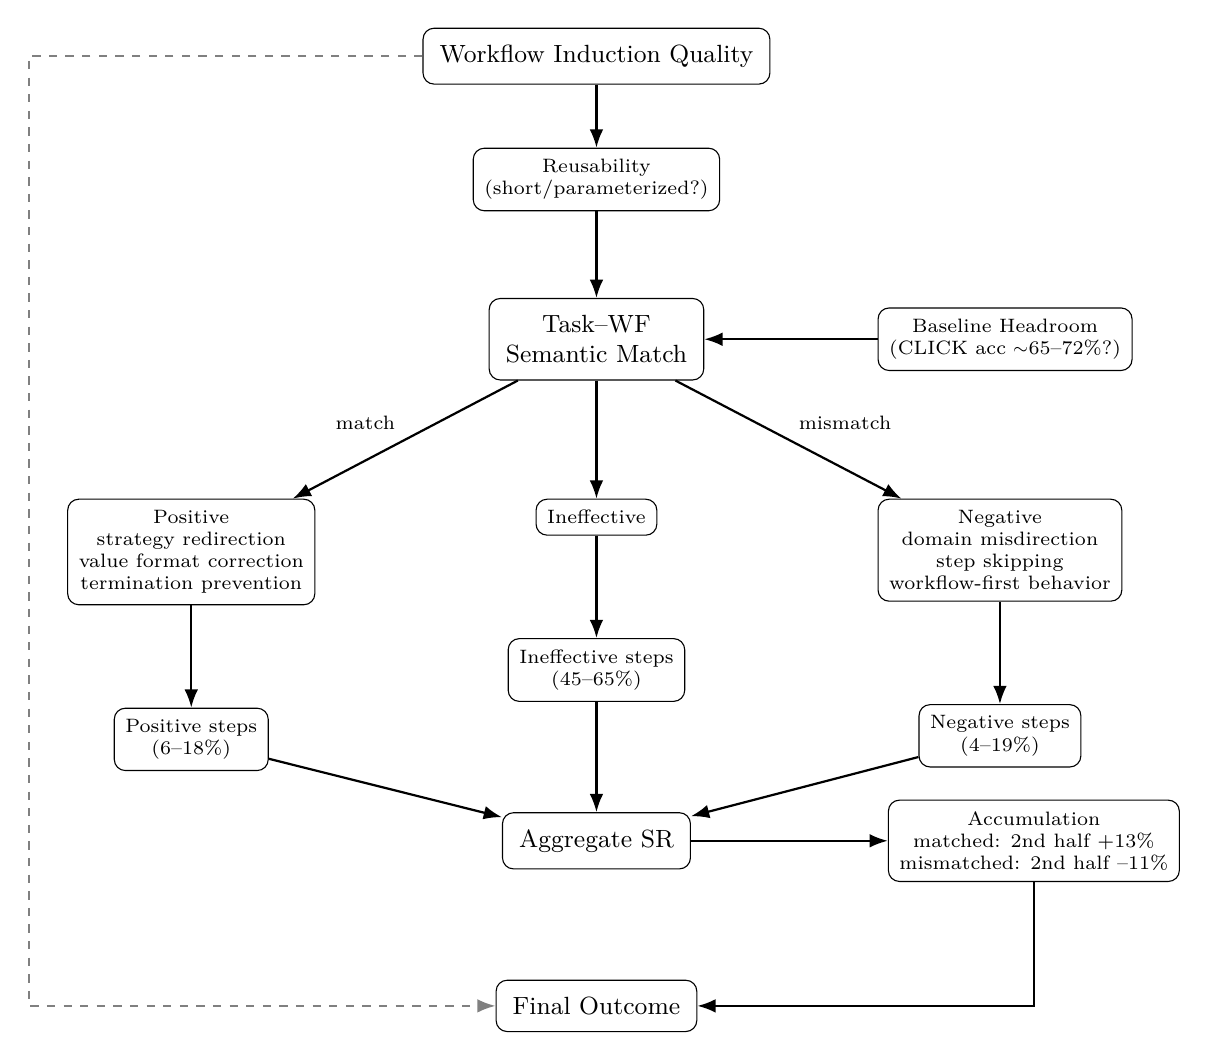
\begin{tikzpicture}[
  >=Latex,
  node distance=1.2cm and 1.7cm,
  box/.style={draw, rounded corners, align=center, inner sep=6pt, font=\small},
  tinybox/.style={draw, rounded corners, align=center, inner sep=4pt, font=\scriptsize},
  flow/.style={->, thick},
  spine/.style={->, thick, dashed, gray}
]

\node[box] (quality) {Workflow Induction Quality};

\node[tinybox, below=0.8cm of quality] (reuse)
  {Reusability\\(short/parameterized?)};

\node[box, below=1.1cm of reuse] (match)
  {Task--WF\\Semantic Match};
\node[tinybox, right=2.2cm of match] (headroom)
  {Baseline Headroom\\(CLICK acc $\sim$65--72\%?)};

\node[tinybox, below left=1.5cm and 2.2cm of match] (pos)
  {Positive\\strategy redirection\\value format correction\\termination prevention};
\node[tinybox, below=1.5cm of match] (ineff)
  {Ineffective};
\node[tinybox, below right=1.5cm and 2.2cm of match] (neg)
  {Negative\\domain misdirection\\step skipping\\workflow-first behavior};

\node[tinybox, below=1.3cm of pos]   (posstep)
  {Positive steps\\(6--18\%)};
\node[tinybox, below=1.3cm of ineff] (ineffstep)
  {Ineffective steps\\(45--65\%)};
\node[tinybox, below=1.3cm of neg]   (negstep)
  {Negative steps\\(4--19\%)};

\node[box, below=1.4cm of ineffstep] (sr)
  {Aggregate SR};

\node[tinybox, right=2.5cm of sr] (accu)
  {Accumulation\\matched: 2nd half +13\%\\mismatched: 2nd half --11\%};

\node[box, below=1.4cm of sr] (outcome)
  {Final Outcome};

\draw[flow] (quality) -- (reuse);
\draw[flow] (reuse)   -- (match);
\draw[flow] (headroom) -- (match);
\draw[flow] (match) -- node[above left,  font=\scriptsize]{match}    (pos);
\draw[flow] (match) -- (ineff);
\draw[flow] (match) -- node[above right, font=\scriptsize]{mismatch} (neg);
\draw[flow] (pos)   -- (posstep);
\draw[flow] (ineff) -- (ineffstep);
\draw[flow] (neg)   -- (negstep);
\draw[flow] (posstep)  -- (sr);
\draw[flow] (ineffstep) -- (sr);
\draw[flow] (negstep)  -- (sr);
\draw[flow] (sr)   -- (accu);
\draw[flow] (accu.south) |- (outcome.east);
\draw[spine] (quality.west) -- ++(-5,0) |- (outcome.west);

\end{tikzpicture}%
}
\caption{Interpretive framework of AWM effects.}
\label{fig:interpretive-framework}
\end{figure}

{\begin{longtable}[]{@{}
  >{\raggedright\arraybackslash}p{(\linewidth - 4\tabcolsep) * \real{0.3200}}
  >{\raggedright\arraybackslash}p{(\linewidth - 4\tabcolsep) * \real{0.3800}}
  >{\raggedright\arraybackslash}p{(\linewidth - 4\tabcolsep) * \real{0.3000}}@{}}
\caption{Paper narrative vs.~observed mechanism.}\label{tab:paper-narrative-vs-observed-mechanism}\\

\toprule\noalign{}
\begin{minipage}[b]{\linewidth}\raggedright
Paper Narrative
\end{minipage} & \begin{minipage}[b]{\linewidth}\raggedright
Observed Mechanism
\end{minipage} & \begin{minipage}[b]{\linewidth}\raggedright
Evidence Status in the Current First-Run Setting
\end{minipage} \\
\midrule\noalign{}
\endhead
\bottomrule\noalign{}
\endlastfoot
AWM is broadly effective & Conditionally effective: requires workflow
reusability + baseline headroom & Exploratory (4-site post-hoc) \\
Online AWM superior under larger gap & Current first-run target-site
results do not reproduce that trend & Direct first-run support \\
Workflow provides ``high-level guidance'' & Workflow changes behavior on
a small fraction of steps via specific mechanisms & Direct first-run
support \\
LM induction better than rule & Abstractness advantage depends on
task-train divergence & Text-level direct support; performance-level
exploratory \\
High utility rate & Prompt-level utility high; behavioral adherence much
lower & Direct first-run support for prompt-level utility; behavioral
adherence exploratory \\
\end{longtable}
}

\section{Design Implications and Proposed
Refinements}\label{design-implications-and-proposed-refinements}

The refinements below constitute this study's design-level
contribution. They are method-design implications drawn from audited
failures, not empirically validated fixes.

The audited negative mechanisms also suggest where a revised AWM
pipeline might intervene more carefully. One useful detail from the
released Mind2Web codebase is that part of the needed machinery already
exists: \texttt{workflow/retrieve.py} implements task-conditioned
semantic retrieval over workflow files using FAISS and OpenAI
embeddings. That retrieval path is not used in the default run loop,
however. Instead, \texttt{run\_mind2web.py} calls
\texttt{memory.py:get\_exemplars}, which reads the entire
\texttt{workflow\_path} file and injects it verbatim into every prompt,
with no per-task filtering, while \texttt{online\_induction.py}
re-induces from all prefix result JSONs without a success filter. The
proposals below therefore map each audited negative case to a concrete
intervention that remains close to the code paths actually exercised in
this reproduction.

{\begin{longtable}[]{@{}
  >{\raggedright\arraybackslash}p{(\linewidth - 6\tabcolsep) * \real{0.18}}
  >{\raggedright\arraybackslash}p{(\linewidth - 6\tabcolsep) * \real{0.27}}
  >{\raggedright\arraybackslash}p{(\linewidth - 6\tabcolsep) * \real{0.22}}
  >{\raggedright\arraybackslash}p{(\linewidth - 6\tabcolsep) * \real{0.33}}@{}}
\caption{Observed failure cases mapped to ideal interventions grounded
in the released Mind2Web code paths.}\label{tab:ideal-interventions}\\

\toprule\noalign{}
\begin{minipage}[b]{\linewidth}\raggedright
Audited case
\end{minipage} & \begin{minipage}[b]{\linewidth}\raggedright
Observed failure
\end{minipage} & \begin{minipage}[b]{\linewidth}\raggedright
Current code path
\end{minipage} & \begin{minipage}[b]{\linewidth}\raggedright
Ideal intervention
\end{minipage} \\
\midrule\noalign{}
\endhead
\bottomrule\noalign{}
\endlastfoot
\textbf{B4} SixFlags jobs (§6.4 N-2) &
Park-navigation workflow is injected for a Jobs task and redirects the
first click to \texttt{Browse the Parks Below} &
\texttt{memory.py:get\_exemplars} reads the full \texttt{workflow\_path}
file and injects it verbatim; no per-task filtering &
\textbf{Task-conditioned workflow retrieval:} wire the semantic mode
of \texttt{workflow/retrieve.py} into \texttt{get\_exemplars}, so that
only the top-\(k\) workflows most similar to \texttt{confirmed\_task}
are injected. In this kind of case, a Jobs-related query would ideally
retrieve no park-navigation workflow above the similarity cutoff. \\
\textbf{N-1} Budget insurance (§6.4) &
Car-rental location-search workflow is injected for an insurance
certificate task and triggers an early zip-code \texttt{TYPE} &
Same as above &
\textbf{Low-similarity no-workflow fallback:} extend the retrieval
step with a similarity threshold \(\tau\); when
\(\max\mathrm{sim}(\text{task}, \text{workflows}) < \tau\), inject no
workflow for that task. This would turn a mismatch from an active harm
channel into a null effect. \\
\textbf{B5} SixFlags template step-skip (§6.4 N-3) &
2-step \texttt{buy\_group\_tickets} template is mapped to a later UI
state, causing the agent to skip date selection and click
\texttt{Book Now} &
Workflow text is treated as a flat string; no step-level precondition
check against the current observation &
\textbf{Workflow-step precondition gating:} before emitting a
workflow step into the prompt, compare its declared element type
(\texttt{[button]}, \texttt{[input]}, \texttt{[select]}) against the
types of the currently visible candidate elements. Workflow steps
whose precondition does not match the current DOM state could then be
suppressed from the injected text. \\
\textbf{B6} TripAdvisor step-0 (Appendix~\ref{app:B6}) &
\texttt{online\_wf} first action produces \texttt{TYPE [search]}
instead of the correct category \texttt{CLICK} at step 0 &
\texttt{online\_induction.py} induces from \emph{all} prefix result
JSONs regardless of outcome; \texttt{memory.py} injects resulting text
uniformly, including at step 0 &
\textbf{Success-gated induction + position- and action-class-aware
gate:} filter the prefix result JSONs inside
\texttt{online\_induction.py} by a success criterion before induction,
bringing the Mind2Web pipeline closer to the paper-level description.
At runtime, when the workflow's leading step suggests an action class
(e.g., \texttt{TYPE} into a search box) that does not match the most
salient visible candidates at step 0, workflow injection for that step
could be suppressed. \\
\end{longtable}
}

These are method-design implications drawn from the observed failures
under the current setting, not validated fixes. The retrieval primitive
in \texttt{workflow/retrieve.py} already exists but is not wired into
the default Mind2Web pipeline; the other interventions (precondition
gating, success-gated induction, position-aware gate) would require new
logic beyond what the released codebase currently provides. Whether any
of them would convert a negative case into an ineffective or positive
one remains an empirical question. What the present analysis can
support is the narrower claim that each proposed intervention targets a
specific, documented failure channel rather than a hypothetical one.

\section{Offline vs Online
Trade-Off}\label{offline-vs-online-trade-off}

The original paper verbally frames offline and online induction as a
trade-off, but does not operationalize that distinction. Our results
sharpen this contrast.

{\begin{longtable}[]{@{}lrrr@{}}
\caption{Offline vs.~online mechanism comparison on kayak.}\label{tab:offline-vs-online-mechanism-comparison-on-kay}\\

\toprule\noalign{}
Delta vs.~no\_workflow & CLICK \ensuremath{\Delta}SR & TYPE \ensuremath{\Delta}ActF1 & TYPE \ensuremath{\Delta}SR \\
\midrule\noalign{}
\endhead
\bottomrule\noalign{}
\endlastfoot
offline\_wf & +10.7\% & +1.4\% & +0.0\% \\
online\_wf & +7.1\% & +19.2\% & +16.7\% \\
\end{longtable}
}

\begin{itemize}
\tightlist
\item
  \textbf{Offline workflows} look like a broad operation library induced
  from training data. On kayak, they are stronger on CLICK-side
  grounding. They contain general travel-search primitives
  (\texttt{enter\ location}, \texttt{select\ travel\ dates},
  \texttt{select\ hotel\ filters}).
\item
  \textbf{Online workflows} look like compressed routines induced from
  recent trajectories. On kayak, they are stronger on
  TYPE/value guidance. They contain narrower, trajectory-shaped routines
  (\texttt{search\_for\_cars\_kayak}, \texttt{select\_location\_kayak}).
\end{itemize}

This means offline vs online should not be interpreted as a simple
ranking:

\begin{itemize}
\tightlist
\item
  Offline is \textbf{broader and steadier}, at least in the current
  `kayak` first-run contrast.
\item
  Online is \textbf{more test-proximate} on `kayak`, but the additional
  target-site readings should be treated as exploratory context rather
  than a standalone mechanism proof.
\end{itemize}

That is a much more precise reading than simply saying ``online helps
more under larger gap.'' Appendix~\ref{app:A7} collects the supporting
trade-off evidence.

\section{Small-Data Efficiency}\label{small-data-efficiency}

The paper implies that online memory can become useful with only a small
number of examples. The current evidence suggests that this is
\textbf{conditionally true}.

{\begin{longtable}[]{@{}llll@{}}
\caption{Online workflow prefix-level Step SR deltas.}\label{tab:online-workflow-prefix-level-step-sr-deltas}\\

\toprule\noalign{}
Site & Earliest Positive Prefix & Best Prefix & Final Prefix \\
\midrule\noalign{}
\endhead
\bottomrule\noalign{}
\endlastfoot
kayak & budget=1, +5.00pp & budget=5, +5.63pp & +5.63pp \\
tripadvisor & none & best still negative & -11.74pp \\
reddit & budget=10, +2.02pp & budget=10, +2.02pp & -2.16pp \\
\end{longtable}
}

\begin{itemize}
\tightlist
\item
  On kayak, a real early gain appears after just one induced example.
\item
  On tripadvisor, there is no early gain at any prefix --- the first
  induced example already introduces bias.
\item
  On reddit, the signal is delayed and unstable.
\end{itemize}

The right conclusion is not that the small-data story is simply false,
but that it is \textbf{conditional in the current first-run evidence}.
Early gains appear on `kayak`, but the same prefix-level pattern is not
reproduced on `tripadvisor` or `reddit`. Appendix~\ref{app:A8}
provides the prefix-level evidence block.

\section{Site Features, Reusability, and
Composition}\label{site-features-reusability-and-composition}

\subsection{Structural Comparison}\label{structural-comparison}

{\begin{longtable}[]{@{}
  >{\raggedright\arraybackslash}p{(\linewidth - 8\tabcolsep) * \real{0.2000}}
  >{\raggedright\arraybackslash}p{(\linewidth - 8\tabcolsep) * \real{0.2000}}
  >{\raggedright\arraybackslash}p{(\linewidth - 8\tabcolsep) * \real{0.2000}}
  >{\raggedright\arraybackslash}p{(\linewidth - 8\tabcolsep) * \real{0.2000}}
  >{\raggedright\arraybackslash}p{(\linewidth - 8\tabcolsep) * \real{0.2000}}@{}}
\caption{Site-level structural comparison.}\\

\toprule\noalign{}
\begin{minipage}[b]{\linewidth}\raggedright
Dimension
\end{minipage} & \begin{minipage}[b]{\linewidth}\raggedright
kayak (positive outcome)
\end{minipage} & \begin{minipage}[b]{\linewidth}\raggedright
newegg (positive outcome)
\end{minipage} & \begin{minipage}[b]{\linewidth}\raggedright
budget (negative outcome)
\end{minipage} & \begin{minipage}[b]{\linewidth}\raggedright
sixflags (negative outcome)
\end{minipage} \\
\midrule\noalign{}
\endhead
\bottomrule\noalign{}
\endlastfoot
Step SR delta & +6.3\% & +5.7\% & -6.1\% & -4.7\% \\
Baseline CLICK acc & 71.4\% & 66.7\% & 63.8\% & 73.5\% \\
AWM CLICK delta & +10.7\% & +6.1\% & -12.1\% & -6.1\% \\
Avg steps/WF & 2.1 & 3.2 & 5.8 & 3.6 \\
WF-task alignment & Strong & Strong & Weak & Partial to Weak \\
\end{longtable}\label{tab:site-level-structural-comparison}
}

The qualitative coding behind these structural rows is documented in
Appendix~\ref{app:C4}.

\subsection{Alignment Rate
(Exploratory)}\label{alignment-rate-exploratory}

An exploratory keyword-overlap heuristic measuring workflow-target
surface alignment yields a counter-intuitive pattern:

{\begin{longtable}[]{@{}lrl@{}}
\caption{Alignment rate vs.~cross-task outcome.}\label{tab:alignment-rate-vs-cross-task-outcome}\\

\toprule\noalign{}
Site & Alignment Rate & Cross-task Outcome \\
\midrule\noalign{}
\endhead
\bottomrule\noalign{}
\endlastfoot
budget & 97.2\% & negative \\
sixflags & 94.2\% & negative \\
newegg & 90.9\% & positive \\
kayak & 70.6\% & positive \\
\end{longtable}
}

Surface alignment does not show a positive monotonic relation with
success. Budget and sixflags have high surface alignment because their
workflow templates cover common action-type keywords --- but the test
tasks involve different semantic instances of those keywords. Newegg
(90.9\%, positive outcome) is an explicit exception to any ``higher alignment
= worse'' story. This metric is exploratory and should not be treated as
a causal indicator. Appendix~\ref{app:A6} documents the heuristic and
its boundary conditions.

\subsection{Working Hypothesis: Dual-Condition
Success}\label{working-hypothesis-dual-condition-success}

Based on the first-run four-site evidence, we propose a working
hypothesis (not a validated rule):

\begin{quote}
AWM effectiveness ≈ f(Workflow Reusability × Baseline Improvement
Headroom)
\end{quote}

Both conditions appear necessary:

\begin{enumerate}
\def\labelenumi{\arabic{enumi}.}
\tightlist
\item
  \textbf{Workflow reusability}: Short, parameterized sub-routines that
  can match multiple test tasks. Kayak/NewEgg satisfy this (2--3
  steps/WF, fully parameterized); budget does not (5.8 steps/WF,
  domain-specific sequences).
\item
  \textbf{Baseline improvement headroom}: Sites where baseline CLICK
  accuracy is in the mid-range, indicating room for element-grounding
  assistance. SixFlags (73.5\% baseline CLICK) already performs well
  without help.
\end{enumerate}

This is a post-hoc observation from four sites, not a validated
threshold.

\subsection{Compositionality on
Mind2Web}\label{compositionality-on-mind2web}

The paper highlights workflow composition as a key capability, showing
how simple workflows combine into more complex ones on WebArena. On
Mind2Web, our reading of the workflow texts reveals a flatter picture:

\begin{itemize}
\tightlist
\item
  \textbf{Explicit hierarchical composition} (one workflow calling
  another): not observed in any Mind2Web workflow file.
\item
  \textbf{Flat subflow reuse} (tasks completed by chaining short
  reusable routines): clearly present on kayak and united, where 1--4
  step parameterized primitives can be flexibly combined.
\item
  \textbf{Template bundling} (long, site-specific sequences serving as
  reusable units only in a weak sense): visible on budget.
\end{itemize}

On Mind2Web, AWM shows signs of subflow reuse mainly as a flat library
of reusable routines, not as explicit hierarchical workflow composition.
This makes the paper's composition narrative partially visible but
considerably weaker and flatter than the WebArena-based narrative
suggests. Appendix~\ref{app:C5} provides the
source-based reading behind this interpretation.

\section{Failure Taxonomy}\label{failure-taxonomy}

The taxonomy below summarizes recurring failure patterns observed under
the current Mind2Web first-run setting. It should be read as a
provisional analytic summary rather than as a validated or exhaustive
ontology: the severity labels reflect the magnitude of impact in the
audited evidence, not a quantified frequency estimate.

The analysis identifies a richer failure taxonomy than the paper
discusses.

{\begin{longtable}[]{@{}
  >{\raggedright\arraybackslash}p{(\linewidth - 6\tabcolsep) * \real{0.2955}}
  >{\raggedright\arraybackslash}p{(\linewidth - 6\tabcolsep) * \real{0.2955}}
  >{\raggedright\arraybackslash}p{(\linewidth - 6\tabcolsep) * \real{0.2273}}
  >{\raggedright\arraybackslash}p{(\linewidth - 6\tabcolsep) * \real{0.1818}}@{}}
\caption{Failure taxonomy.}\\

\toprule\noalign{}
\begin{minipage}[b]{\linewidth}\raggedright
Failure Mode
\end{minipage} & \begin{minipage}[b]{\linewidth}\raggedright
Description
\end{minipage} & \begin{minipage}[b]{\linewidth}\raggedright
Severity
\end{minipage} & \begin{minipage}[b]{\linewidth}\raggedright
Source
\end{minipage} \\
\midrule\noalign{}
\endhead
\bottomrule\noalign{}
\endlastfoot
\textbf{Workflow mismatch} & Workflow template does not apply to current
step, redirecting agent away from correct action & High & §5.2, §6.4 \\
\textbf{Target-site first-run underperformance} & Current target-site
results show wrong early action patterns and weaker candidate quality in
some settings; this remains result tracing rather than standalone
mechanism proof & High & §5.3 \\
\textbf{Cumulative misdirection} & Workflow harm amplifies in the second
half of trajectories & Medium & §5.2.2 \\
\textbf{Over-specificity} & Rule workflows preserve too many source-site
concrete values & Medium & §5.4.2 \\
\textbf{Representation noise} & Mixed desc\_html representation
increases prompt length and dilutes attention & Medium & §5.5.2 \\
\textbf{Workflow ineffectiveness} & Workflow exists but does not affect
model output (45--65\% of steps) & Low & §5.2.3 \\
\textbf{SKIP-step inflation} & Ground truth elements absent from
candidates, inflating failure counts across all conditions & Structural
& §5.2 \\
\textbf{Limited coverage} & 5--7 abstract workflows cannot cover all
test-step operation types & Structural & §5.6 \\
\end{longtable}
\label{tab:failure-taxonomy-main}
}

These failures are not all the same type. Some come from workflow
mismatch, some from candidate quality, some from sparse coverage, and
some from prompt-structure effects. The paper does not discuss any of
them.

\section{Overall Assessment}\label{overall-assessment}

\subsection{Main Supported Findings}\label{what-is-reproduced}

Within the current Mind2Web first-run setting and under the present
GPT-4o / Qwen backbones, the strongest supported conclusions are:

\begin{itemize}
\tightlist
\item
  LM-induced workflows are more abstract than rule-induced ones (4/4
  text-level indicators, all three sites).
\item
  Prompt-level code and text workflow representations behave similarly
  on the tested site.
\item
  Workflow libraries are compact and low-overlap.
\item
  In the audited matched-site cases, workflows improve local
  step-level execution with zero negative interventions.
\end{itemize}

\subsection{Main Unsupported
Claims}\label{what-is-not-reproduced}

Within the same setting, the current Mind2Web evidence does not
support:

\begin{itemize}
\tightlist
\item
  Online AWM becoming stronger under larger distribution gap.
\item
  Natural-language observations being generally better than HTML.
\item
  A uniformly site-robust reading of AWM.
\end{itemize}

\subsection{What Becomes More
Precise}\label{what-becomes-more-precise}

Within the current Mind2Web first-run setting and under the present
GPT-4o / Qwen backbones, the paper's broadest claims can be
rewritten more carefully:

\begin{itemize}
\tightlist
\item
  On the seven sites audited here, AWM is not uniformly effective.
  Under this envelope, the most accurate description is
  \textbf{conditionally effective}, with that condition still bounded
  by backbone-specific and single-run caveats.
\item
  On the audited sites, workflow usefulness is sparse rather than
  pervasive in the first run, changing behavior on only 6--18\% of
  steps.
\item
  On the two target sites evaluated here (\texttt{tripadvisor} and
  \texttt{reddit}), online memory is not broadly superior under shift
  in the first run; the narrower reading supported here is that it
  appears \textbf{more test-proximate yet more brittle} in these
  cases, pending repeated trials.
\item
  Under these conditions, abstraction helps on the sites where
  workflow reusability aligns with task-family operations; the
  present evidence does not establish this as a universal law.
\item
  In the audited matched-site cases, AWM's gains come from specific
  mechanisms (strategy redirection, value guidance, termination
  prevention) rather than from generic ``high-level operational
  guidance.''
\end{itemize}

\section{Threats to Validity}\label{threats-to-validity}

This study has six main limitations.

\begin{enumerate}
\def\labelenumi{\arabic{enumi}.}
\item
  \textbf{Mind2Web only.} The paper also reports WebArena results, which
  are outside the present scope. Some of the paper's stronger narratives
  (especially around workflow composition) are primarily supported by
  WebArena evidence. This also means the flatter Mind2Web
  compositionality reading in §\ref{compositionality-on-mind2web} cannot
  be contrasted directly against the WebArena evidence on which the
  paper's stronger composition narrative rests, so a WebArena extension
  remains part of the future-work agenda.
\item
  \textbf{First-run judgments.} The current positive / negative / mixed
  decisions are informative but are not repeated-trial estimates with
  variance bounds. ``Unsupported'' should be read as ``unsupported in
  the current first-run setting,'' not as ``definitively false.''
\item
  \textbf{No AWM\_AS coverage.} The paper's action-space extension
  branch (§5, Table~9) is not covered. This is a scope limitation of
  the current study rather than a contradictory finding.
\item
  \textbf{Exploratory alignment rate.} The alignment-rate measure is
  based on keyword overlap, not semantic matching. It is suitable for
  generating hypotheses but not for causal claims.
\item
  \textbf{Model-generation confound.} The original paper uses
  \textbf{GPT-4} and \textbf{GPT-3.5-turbo}, whereas this reproduction
  uses \textbf{GPT-4o} and \textbf{Qwen}. The present study therefore
  does not isolate method
  effects from backbone effects. Stronger or differently aligned
  models may internalize some of the procedural knowledge that AWM is
  intended to externalize, so site-level ``not reproduced'' patterns
  cannot be cleanly attributed to AWM alone. AWM is intended as a
  model-agnostic mechanism; this limitation is recorded here as an
  evidence boundary rather than as a contradiction of that design
  intent.
\item
  \textbf{Released-code-faithful Mind2Web pipeline.} All online results
  follow the released Mind2Web implementation (see
  §\ref{online-induction}), which re-induces workflows from all
  prefix result JSONs rather than applying an explicit success-only
  filter before induction. Mechanism-level readings of online AWM here
  should therefore be interpreted relative to the released pipeline,
  not to the paper-level success-gated description.
\end{enumerate}

These limitations are part of the study's explicit evidence boundary,
not hidden caveats disclosed only at the end.

\section{Conclusion and Future
Work}\label{conclusion-and-future-work}

\subsection{Summary}\label{summary}

This deep reproduction supports a more qualified picture of AWM than the
original paper presents.

The method shows a real mechanism in the current reproduction setting.
Reusable workflows can improve step-level decisions, especially through
TYPE-side value guidance and matched CLICK-side grounding. LM-induced
workflows are more abstract than rule-induced ones at the text level,
and workflow libraries are compact. These are the parts of the paper's
story best supported by the present evidence.

At the same time, in the current first-run evidence, the reproduction
does not support the strongest version of the paper's performance
narrative. Online AWM does not become more reliable under larger
distribution shift on the tested Mind2Web settings. The NL-over-HTML
claim also does not generalize in the three-site evaluation. AWM's gains
are sparse, site-dependent, and highly contingent on workflow--task
match.

The most defensible final judgment is therefore, under the present
experimental envelope (Mind2Web only, first-run, GPT-4o and Qwen,
released-code-faithful pipeline):
\textbf{AWM is a plausible and interpretable prompting mechanism in
this reproduction setting, but the present evidence does not support a
uniformly reliable memory method. Its core idea survives reproduction
better than its strongest universality claims, yet the conclusion
remains conditional on the setting envelope and on single-run
evidence.}

Relative to the procedural-memory gap identified in the Interim report,
AWM is best read as a partial rather than complete solution: it
operationalizes post-task workflow reuse, but lacks the failure-driven
write-back mechanism that the Interim identified as equally
load-bearing.

That is precisely what a critical reproduction should reveal under
these conditions.

\subsection{Future Work}\label{future-work}

The directions below are ordered by how tightly they close the gaps
identified in the Interim report: failure-driven workflow revision and
semantic workflow selection directly address the primary
procedural-memory and failure-driven write-back gaps, while the
remaining items broaden the current evidence envelope.

\begin{enumerate}
\def\labelenumi{\arabic{enumi}.}
\item
  \textbf{Repeated trials with variance estimation.} Converting
  first-run judgments into statistically grounded conclusions requires
  multiple runs with different random seeds and confidence intervals.
\item
  \textbf{Failure-driven workflow revision.} AWM currently has no
  mechanism for revising or retracting workflows that cause harm. A
  write-back loop that detects harmful patterns and modifies or removes
  offending workflows could address the method's most severe failure
  mode.
\item
  \textbf{Semantic workflow selection.} The current approach injects all
  workflows uniformly. A retrieval mechanism that selects workflows
  based on task-workflow semantic similarity could reduce
  mismatch-induced harm.
\item
  \textbf{WebArena reproduction.} Extending the analysis to WebArena
  would test whether the boundary conditions identified here are
  Mind2Web-specific or structural properties of AWM.
\item
  \textbf{Cross-model robustness.} Testing with a wider range of
  backbone models would help distinguish method-level properties from
  model-specific behaviors.
\end{enumerate}

\section{References}\label{references}

\printbibliography[heading=none]

\clearpage
\appendix
\section{Appendix}\label{appendix}

\setcounter{table}{0}
\renewcommand{\thetable}{A\arabic{table}}

{\small
\setlength{\tabcolsep}{5pt}
\renewcommand{\arraystretch}{1.15}
\setlength{\LTleft}{0pt}
\setlength{\LTright}{0pt}
% A1
\subsection{Step-Level Breakdown Evidence}\label{app:A1}

This appendix supports step-level claims about where AWM gains and
losses come from in \texttt{C1}. The evidence below is drawn from the
audited step-level decomposition of the \texttt{C1} sites.

\subsubsection{Representative step-level deltas from the source
output}

{\def\LTcaptype{} % do not increment counter
\begin{longtable}[]{@{}>{\raggedright\arraybackslash}p{0.14\linewidth}>{\raggedright\arraybackslash}p{0.22\linewidth}>{\raggedleft\arraybackslash}p{0.14\linewidth}>{\raggedleft\arraybackslash}p{0.14\linewidth}>{\raggedleft\arraybackslash}p{0.14\linewidth}>{\raggedleft\arraybackslash}p{0.18\linewidth}@{}}
\toprule\noalign{}
Website & Condition & \texttt{CLICK\ dElem\ /\ dStepSR} &
\texttt{TYPE\ dElem\ /\ dActF1\ /\ dStepSR} &
\texttt{first\_half\ dStepSR} & \texttt{second\_half\ dStepSR} \\
\midrule\noalign{}
\endhead
\bottomrule\noalign{}
\endlastfoot
\texttt{budget} & \texttt{offline\_wf\ -\ no\_workflow} &
\texttt{-12.1\ /\ -12.1} & \texttt{+0.0\ /\ +8.4\ /\ +9.1} &
\texttt{-1.9} & \texttt{-10.9} \\
\texttt{kayak} & \texttt{offline\_wf\ -\ no\_workflow} &
\texttt{+10.7\ /\ +10.7} & \texttt{+0.0\ /\ +1.4\ /\ +0.0} &
\texttt{+0.0} & \texttt{+13.0} \\
\texttt{newegg} & \texttt{offline\_wf\ -\ no\_workflow} &
\texttt{+9.1\ /\ +6.1} & \texttt{+33.3\ /\ +50.0\ /\ +33.3} &
\texttt{+4.4} & \texttt{+7.1} \\
\texttt{sixflags} & \texttt{offline\_wf\ -\ no\_workflow} &
\texttt{-6.1\ /\ -6.1} & \texttt{+0.0\ /\ +0.0\ /\ +0.0} & \texttt{-5.9}
& \texttt{-3.3} \\
\texttt{united} & \texttt{offline\_wf\ -\ no\_workflow} &
\texttt{+3.6\ /\ +3.6} & \texttt{+16.7\ /\ +2.8\ /\ +0.0} &
\texttt{+3.0} & \texttt{+0.0} \\
\texttt{yellowpages} & \texttt{offline\_wf\ -\ no\_workflow} &
\texttt{+0.0\ /\ +0.0} & \texttt{+28.6\ /\ +19.5\ /\ +28.6} &
\texttt{+0.0} & \texttt{+7.1} \\
\end{longtable}
}

\subsubsection{Source excerpts}

\paragraph{Kayak}

\begin{verbatim}
[Delta: offline_wf - no_workflow] by action_type
  CLICK                   +10.7%     +3.6%    +10.7%
  SKIP                     +0.0%     +0.0%     +0.0%
  TYPE                     +0.0%     +1.4%     +0.0%

[Delta: offline_wf - no_workflow] by step_half
  first_half               +0.0%     +0.3%     +0.0%
  second_half             +13.0%     +4.3%    +13.0%
\end{verbatim}

\paragraph{Budget}

\begin{verbatim}
[Delta: offline_wf - no_workflow] by action_type
  CLICK                   -12.1%     -1.7%    -12.1%
  SELECT                   +0.0%     +0.0%     +0.0%
  SKIP                     +0.0%     +0.0%     +0.0%
  TYPE                     +0.0%     +8.4%     +9.1%

[Delta: offline_wf - no_workflow] by step_half
  first_half               -3.8%     +3.6%     -1.9%
  second_half             -10.9%     -4.3%    -10.9%
\end{verbatim}

\paragraph{Newegg}

\begin{verbatim}
[Delta: offline_wf - no_workflow] by action_type
  CLICK                    +9.1%     -3.0%     +6.1%
  SELECT                   +0.0%    +20.0%    +25.0%
  SKIP                     +0.0%     +0.0%     +0.0%
  TYPE                    +33.3%    +50.0%    +33.3%
\end{verbatim}

\subsubsection{Interpretation limits}

\begin{itemize}
\tightlist
\item
  This appendix supports direction-of-effect claims, not causal proof.
\item
  \texttt{TYPE} counts are small on several sites, so the main robust
  use is qualitative: \texttt{TYPE} gains are often non-negative while
  \texttt{CLICK} varies sharply by site.
\item
  Later-step accumulation is strongest on \texttt{kayak}; other sites
  show weaker or mixed support.
\end{itemize}


% A2
\clearpage
\subsection{Paired-Case Summary Evidence}\label{app:A2}

This appendix supports claims about how often workflow actually changes
behavior, and whether changed steps are net positive or net negative.
The evidence below summarizes the audited paired-case distributions over
the seven \texttt{C1} sites.

\subsubsection{\texorpdfstring{A2.1 Corrected overall totals for the seven
\texttt{C1}
websites}{A2.1 Corrected overall totals for the seven C1 websites}}

This table corrects the earlier erroneous denominator \texttt{523}.\\
The total paired-step count for the seven audited \texttt{C1} sites is
\texttt{475}.

{\def\LTcaptype{} % do not increment counter
\begin{longtable}[]{@{}>{\raggedright\arraybackslash}p{0.28\linewidth}>{\raggedright\arraybackslash}p{0.46\linewidth}>{\raggedright\arraybackslash}p{0.22\linewidth}@{}}
\toprule\noalign{}
Category & Count & Pct of all paired steps \\
\midrule\noalign{}
\endhead
\bottomrule\noalign{}
\endlastfoot
\texttt{positive} & 26 & \texttt{5.5\%} \\
\texttt{negative} & 24 & \texttt{5.1\%} \\
\texttt{ineffective} & 252 & \texttt{53.1\%} \\
\texttt{redundant} & 173 & \texttt{36.4\%} \\
\texttt{changed\ =\ positive\ +\ negative} & 50 & \texttt{10.5\%} \\
\end{longtable}
}

Among changed steps only:

{\def\LTcaptype{} % do not increment counter
\begin{longtable}[]{@{}>{\raggedright\arraybackslash}p{0.36\linewidth}>{\centering\arraybackslash}p{0.60\linewidth}@{}}
\toprule\noalign{}
Metric & Value \\
\midrule\noalign{}
\endhead
\bottomrule\noalign{}
\endlastfoot
\texttt{positive\ /\ (positive\ +\ negative)} &
\texttt{26\ /\ 50\ =\ 52.0\%} \\
\texttt{net\ gain} & \texttt{+2\ steps} \\
\end{longtable}
}

\subsubsection{\texorpdfstring{A2.2 Site-wise evidence from
\texttt{C1}}{A2.2 Site-wise evidence from C1}}

{\def\LTcaptype{} % do not increment counter
\begin{longtable}[]{@{}>{\raggedright\arraybackslash}p{0.12\linewidth}>{\raggedleft\arraybackslash}p{0.20\linewidth}>{\raggedleft\arraybackslash}p{0.11\linewidth}>{\raggedleft\arraybackslash}p{0.11\linewidth}>{\raggedleft\arraybackslash}p{0.11\linewidth}>{\raggedleft\arraybackslash}p{0.11\linewidth}>{\raggedright\arraybackslash}p{0.20\linewidth}@{}}
\toprule\noalign{}
Website & Total & Positive & Negative & Ineffective & Redundant &
Verdict pattern \\
\midrule\noalign{}
\endhead
\bottomrule\noalign{}
\endlastfoot
\texttt{budget} & 99 & 6 & 12 & 53 & 28 & negative-dominated \\
\texttt{kayak} & 48 & 3 & 0 & 22 & 23 & reproduced, no negatives \\
\texttt{kohls} & 53 & 2 & 2 & 33 & 16 & mixed \\
\texttt{newegg} & 87 & 5 & 0 & 56 & 26 & reproduced, no negatives \\
\texttt{sixflags} & 64 & 3 & 6 & 23 & 32 & negative-dominated \\
\texttt{united} & 63 & 3 & 2 & 35 & 23 & slight positive edge \\
\texttt{yellowpages} & 61 & 4 & 2 & 30 & 25 & slight positive edge \\
\end{longtable}
}

\subsubsection{Source excerpts}

\paragraph{Kayak}

\begin{verbatim}
[Overall Distribution]
  positive             3    6.2%
  negative             0    0.0%
  ineffective         22   45.8%
  redundant           23   47.9%

[Workflow Impact]
  Positive / (Positive + Negative) = 3/3 = 100.0%
  Net gain (positive - negative)   = +3 steps
\end{verbatim}

\paragraph{Newegg}

\begin{verbatim}
[Overall Distribution]
  positive             5    5.7%
  negative             0    0.0%
  ineffective         56   64.4%
  redundant           26   29.9%
\end{verbatim}

\paragraph{Budget}

\begin{verbatim}
[Overall Distribution]
  positive             6    6.1%
  negative            12   12.1%
  ineffective         53   53.5%
  redundant           28   28.3%
\end{verbatim}

\paragraph{Sixflags}

\begin{verbatim}
[Overall Distribution]
  positive             3    4.7%
  negative             6    9.4%
  ineffective         23   35.9%
  redundant           32   50.0%
\end{verbatim}

\subsubsection{Interpretation limits}

\begin{itemize}
\tightlist
\item
  This appendix supports statements about behavioral footprint and sign
  of net change.
\item
  It should not be used to claim that all changed steps are equally
  important.
\item
  The corrected denominator \texttt{475} should be used consistently
  wherever these \texttt{C1} distributions are discussed.
\end{itemize}


% A3
\clearpage
\subsection{First-Run Target-Site Result Note}\label{app:A3}

This appendix records the first-run result facts on the two target
sites and preserves the corresponding diagnostic output as exploratory
tracing material. The note below is based on the audited target-site
error summaries and their associated negative-case review.

\subsubsection{Summary table}

{\def\LTcaptype{} % do not increment counter
\begin{longtable}[]{@{}>{\raggedright\arraybackslash}p{0.12\linewidth}>{\raggedright\arraybackslash}p{0.20\linewidth}>{\raggedleft\arraybackslash}p{0.11\linewidth}>{\raggedleft\arraybackslash}p{0.11\linewidth}>{\raggedleft\arraybackslash}p{0.11\linewidth}>{\raggedleft\arraybackslash}p{0.11\linewidth}>{\raggedright\arraybackslash}p{0.20\linewidth}@{}}
\toprule\noalign{}
Target & Model / setup & Positive & Negative & Skip-rate shift vs source
& CLICK share of negatives & Safe reading \\
\midrule\noalign{}
\endhead
\bottomrule\noalign{}
\endlastfoot
\texttt{tripadvisor} & \texttt{qwen/qwen3.5-397b-\allowbreak a17b\ /\ online\_wf} &
4 & 18 & \texttt{+16pp} (\texttt{44.9\%} vs \texttt{29.2\%}) &
\texttt{78\%} & first-run underperformance with weaker baseline
candidate quality \\
\texttt{reddit} & \texttt{qwen/qwen3.5-397b-\allowbreak a17b\ /\ online\_wf} & 2 & 5
& \texttt{+4.7pp} (\texttt{33.9\%} vs \texttt{29.2\%}) & \texttt{80\%} &
first-run underperformance without obvious baseline collapse \\
\end{longtable}
}

\subsubsection{Source excerpts}

\paragraph{Reddit}

\begin{verbatim}
[Degradation Profile: online_wf]
  Positive: 2, Negative: 5, Ineffective: 87, Redundant: 86

[Hypothesis B: Element grounding collapse]
  Skip rate (target baseline): 33.9%
  Skip rate (source baseline): 29.2%
  CLICK Elem Acc (target baseline): 84.2%
  CLICK Elem Acc (source baseline): 75.0%
  -> No strong B evidence (baseline performs similarly)

[Hypothesis A: Workflow content mismatch]
  Negative steps: 5
    CLICK: 4  TYPE: 1
    CLICK share of negatives: 80%
  -> A evidence: Negatives dominated by CLICK (element-level mismatch, not value mismatch)

[Preliminary Verdict]
  -> Primarily Hypothesis A: workflow content is mismatched
\end{verbatim}

\paragraph{Tripadvisor}

\begin{verbatim}
[Degradation Profile: online_wf]
  Positive: 4, Negative: 18, Ineffective: 131, Redundant: 72

[Hypothesis B: Element grounding collapse]
  Skip rate (target baseline): 44.9%
  Skip rate (source baseline): 29.2%
  CLICK Elem Acc (target baseline): 81.2%
  CLICK Elem Acc (source baseline): 75.0%
  -> B evidence: Skip rate +16pp higher on target site

[Hypothesis A: Workflow content mismatch]
  Negative steps: 18
    CLICK: 14  TYPE: 4
    CLICK share of negatives: 78%
  -> A evidence: Negatives dominated by CLICK (element-level mismatch, not value mismatch)

[Preliminary Verdict]
  -> Mixed: both element grounding degradation AND workflow mismatch
\end{verbatim}

\subsubsection{Interpretation limits}

\begin{itemize}
\tightlist
\item
  This appendix is best used as first-run result tracing, not as a
  report-level mechanism proof.
\item
  The diagnostic labels in the underlying output are useful for
  internal inspection, but they should not be promoted to workflow
  provenance claims or full causal decomposition.
\item
  The strongest safe summary is:

  \begin{itemize}
  \tightlist
  \item
    \texttt{tripadvisor}: first-run underperformance plus weaker
    baseline candidate quality
  \item
    \texttt{reddit}: first-run underperformance without obvious
    baseline collapse
  \end{itemize}
\end{itemize}


% A4
\clearpage
\subsection{C4 Result Table}\label{app:A4}

This appendix supports \texttt{C4} claims about \texttt{NL\ vs\ HTML}
and \texttt{code\ vs\ text\ workflow}. The tables below consolidate the
audited first-run \texttt{C4} representation results.

\subsubsection{\texorpdfstring{A4.1 \texttt{NL\ vs\ HTML} first-run
results}{A4.1 NL vs HTML first-run results}}

{\def\LTcaptype{} % do not increment counter
\begin{longtable}[]{@{}>{\raggedright\arraybackslash}p{0.14\linewidth}>{\raggedright\arraybackslash}p{0.22\linewidth}>{\raggedleft\arraybackslash}p{0.14\linewidth}>{\raggedleft\arraybackslash}p{0.14\linewidth}>{\raggedleft\arraybackslash}p{0.14\linewidth}>{\raggedleft\arraybackslash}p{0.18\linewidth}@{}}
\toprule\noalign{}
Website & Condition & Element Acc & Action F1 & Step SR & SR \\
\midrule\noalign{}
\endhead
\bottomrule\noalign{}
\endlastfoot
\texttt{kayak} & \texttt{desc\_only} & 54.8 & 61.2 & 45.3 & 0.0 \\
\texttt{kayak} & \texttt{html\_only} & 52.4 & 63.5 & 48.0 & 0.0 \\
\texttt{kayak} & \texttt{desc\_html} & 54.8 & 63.5 & 50.3 & 0.0 \\
\texttt{united} & \texttt{desc\_only} & 57.9 & 61.9 & 55.9 & 33.3 \\
\texttt{united} & \texttt{html\_only} & 61.2 & 64.5 & 60.6 & 33.3 \\
\texttt{united} & \texttt{desc\_html} & 57.9 & 61.1 & 51.7 & 16.7 \\
\texttt{newegg} & \texttt{desc\_only} & 42.0 & 44.3 & 30.5 & 0.0 \\
\texttt{newegg} & \texttt{html\_only} & 36.2 & 42.6 & 23.9 & 0.0 \\
\texttt{newegg} & \texttt{desc\_html} & 38.0 & 42.4 & 30.3 & 0.0 \\
\end{longtable}
}

\subsubsection{\texorpdfstring{A4.2 \texttt{code\ vs\ text\ workflow}
first-run
result}{A4.2 code vs text workflow first-run result}}

{\def\LTcaptype{} % do not increment counter
\begin{longtable}[]{@{}>{\raggedright\arraybackslash}p{0.14\linewidth}>{\raggedright\arraybackslash}p{0.22\linewidth}>{\raggedleft\arraybackslash}p{0.14\linewidth}>{\raggedleft\arraybackslash}p{0.14\linewidth}>{\raggedleft\arraybackslash}p{0.14\linewidth}>{\raggedleft\arraybackslash}p{0.18\linewidth}@{}}
\toprule\noalign{}
Website & Condition & Element Acc & Action F1 & Step SR & SR \\
\midrule\noalign{}
\endhead
\bottomrule\noalign{}
\endlastfoot
\texttt{kayak} & \texttt{text\_wf} & 55.3 & 60.8 & 45.8 & 0.0 \\
\texttt{kayak} & \texttt{code\_wf} & 52.4 & 63.4 & 48.0 & 0.0 \\
\end{longtable}
}

\subsubsection{Interpretive summary}

The three-site \texttt{NL\ vs\ HTML} comparison does not support the
paper's directional claim on Mind2Web. Under the current prompt-level
code representation, the first \texttt{kayak} run suggests only modest
differences between \texttt{code\ workflow} and
\texttt{text\ workflow}.

\subsubsection{Interpretation limits}

\begin{itemize}
\tightlist
\item
  This appendix supports first-run result claims only.
\item
  \texttt{code\ vs\ text\ workflow} currently has one audited site
  (\texttt{kayak}), not a three-site result.
\end{itemize}


% A5
\clearpage
\subsection{C5 Workflow Quality Table}\label{app:A5}

This appendix supports \texttt{C5} claims about workflow compactness,
overlap, and prompt-level usage proxies. The table below summarizes the
audited first-run workflow-quality statistics under the current
approximation.

\subsubsection{First-run quality
table}

{\def\LTcaptype{} % do not increment counter
\begin{longtable}[]{@{}>{\raggedright\arraybackslash}p{0.12\linewidth}>{\raggedright\arraybackslash}p{0.20\linewidth}>{\raggedleft\arraybackslash}p{0.11\linewidth}>{\raggedleft\arraybackslash}p{0.11\linewidth}>{\raggedleft\arraybackslash}p{0.11\linewidth}>{\raggedleft\arraybackslash}p{0.11\linewidth}>{\raggedright\arraybackslash}p{0.20\linewidth}@{}}
\toprule\noalign{}
Website & Condition & \#workflows & coverage & function overlap &
utility rate & Current verdict \\
\midrule\noalign{}
\endhead
\bottomrule\noalign{}
\endlastfoot
\texttt{kayak} & \texttt{lm\_wf} & 7 & 1.0 & 0.0 & 1.0 &
\texttt{reproduced\ (first\ run)} \\
\texttt{newegg} & \texttt{lm\_wf} & 5 & 1.0 & 0.0333 & 1.0 &
\texttt{reproduced\ (first\ run)} \\
\texttt{united} & \texttt{lm\_wf} & 5 & 1.0 & 0.0 & 1.0 &
\texttt{reproduced\ (first\ run)} \\
\end{longtable}
}

\subsubsection{Interpretive summary}

Across the three audited sites, the first-run evidence supports the
directional workflow-quality conclusion under the current approximation:
the workflow libraries are compact, pairwise overlap is low, and the
prompt-level usage proxies are high. The main caveat is that
\texttt{utility\ rate} remains a broad proxy rather than a strict
adherence measure.

\subsubsection{Interpretation limits}

\begin{itemize}
\tightlist
\item
  \texttt{coverage\ =\ 1.0} and \texttt{utility\ rate\ =\ 1.0} here are
  prompt-level proxies.
\item
  These values should not be reworded as ``the model always followed the
  workflow.''
\item
  The safest wording is: the workflow text was consistently present and
  detectable in the prompt context under the current approximation.
\end{itemize}


% A6
\clearpage
\subsection{Alignment-Rate Note}\label{app:A6}

This appendix provides a traceable source block for the exploratory
alignment-rate numbers used in \texttt{§10.2}. The heuristic below is
reconstructed from the alignment-rate analysis used during the audit.

\subsubsection{What this metric is}

The alignment-rate audit computes a workflow-target alignment heuristic
using keyword overlap between:

\begin{itemize}
\tightlist
\item
  workflow pattern descriptions
\item
  target-element context extracted from the observation HTML
\end{itemize}

It is explicitly \textbf{not} a semantic-match metric.

\subsubsection{Current site-wise
values}

{\def\LTcaptype{} % do not increment counter
\begin{longtable}[]{@{}>{\raggedright\arraybackslash}p{0.28\linewidth}>{\raggedleft\arraybackslash}p{0.46\linewidth}>{\raggedright\arraybackslash}p{0.22\linewidth}@{}}
\toprule\noalign{}
Website & Alignment rate & C1 status \\
\midrule\noalign{}
\endhead
\bottomrule\noalign{}
\endlastfoot
\texttt{budget} & 97.2\% & not reproduced \\
\texttt{sixflags} & 94.2\% & not reproduced \\
\texttt{newegg} & 90.9\% & reproduced \\
\texttt{kayak} & 70.6\% & reproduced \\
\end{longtable}
}

\subsubsection{Safe interpretation}

\begin{itemize}
\tightlist
\item
  The metric is suitable for supporting the claim that \textbf{surface
  alignment does not reliably predict performance}.
\item
  It is \textbf{not} strong enough to support semantic-fit claims on its
  own.
\item
  \texttt{newegg} is an explicit exception to any monotonic ``higher
  alignment = worse performance'' story.
\end{itemize}

\subsubsection{Source excerpt}

\begin{verbatim}
Heuristic: keyword overlap between workflow pattern descriptions
           and observation element context for each target action.
Limitations: label-lag, keyword ambiguity, placeholder fallback,
             no value-level matching for TYPE/SELECT.

SUMMARY TABLE
  kayak               17      6     34       24    70.6%
  newegg              14      7     44       40    90.9%
  budget              35     10     71       69    97.2%
  sixflags            18      7     52       49    94.2%
\end{verbatim}


% A7
\clearpage
\subsection{Offline-vs-Online Trade-Off}\label{app:A7}

\subsubsection{Overview}

This appendix is retained as an exploratory rereading of existing
Mind2Web outputs. It should not be used as a primary final-report
appendix for target-site mechanism claims.

The goal here is not to introduce a new experiment. It is to re-read
existing outputs from a mechanism perspective and ask:

\begin{itemize}
\tightlist
\item
  what kinds of step-level gains does \texttt{offline\_wf} produce on
  \texttt{kayak}?
\item
  what kinds of step-level gains does \texttt{online\_wf} produce on the
  same site?
\item
  what first-run result pattern appears on the farther targets
  \texttt{tripadvisor} and \texttt{reddit}?
\end{itemize}

This appendix is based on four source types: audited step-level
summaries, audited paired-case summaries, workflow texts from
\texttt{kayak}, and manually verified negative cases from the
\texttt{tripadvisor} and \texttt{reddit} target-site runs.

\subsubsection{\texorpdfstring{A7.1 Same-Site Comparison on
\texttt{kayak}}{A7.1 Same-Site Comparison on kayak}}

\paragraph{Aggregate outcome}

From the audited step-level summary:

{\def\LTcaptype{} % do not increment counter
\begin{longtable}[]{@{}>{\raggedright\arraybackslash}p{0.20\linewidth}>{\raggedleft\arraybackslash}p{0.30\linewidth}>{\raggedleft\arraybackslash}p{0.22\linewidth}>{\raggedleft\arraybackslash}p{0.24\linewidth}@{}}
\toprule\noalign{}
condition & Elem Acc & Act F1 & Step SR \\
\midrule\noalign{}
\endhead
\bottomrule\noalign{}
\endlastfoot
no\_workflow & 52.1\% & 60.9\% & 47.9\% \\
offline\_wf & 58.3\% & 63.2\% & 54.2\% \\
online\_wf & 56.2\% & 65.4\% & 54.2\% \\
\end{longtable}
}

Observation:

\begin{itemize}
\tightlist
\item
  both \texttt{offline\_wf} and \texttt{online\_wf} improve
  \texttt{Step\ SR} by \texttt{+6.3pp} over baseline on \texttt{kayak}
\item
  \texttt{offline\_wf} has slightly higher \texttt{Elem\ Acc}
\item
  \texttt{online\_wf} has slightly higher \texttt{Act\ F1}
\end{itemize}

This already suggests that the two conditions are not helping in exactly
the same way.

\paragraph{Action-type
decomposition}

From the audited step-level summary:

{\def\LTcaptype{} % do not increment counter
\begin{longtable}[]{@{}>{\raggedright\arraybackslash}p{0.20\linewidth}>{\raggedleft\arraybackslash}p{0.30\linewidth}>{\raggedleft\arraybackslash}p{0.22\linewidth}>{\raggedleft\arraybackslash}p{0.24\linewidth}@{}}
\toprule\noalign{}
delta vs no\_workflow & CLICK dStepSR & TYPE dActF1 & TYPE dStepSR \\
\midrule\noalign{}
\endhead
\bottomrule\noalign{}
\endlastfoot
offline\_wf & +10.7\% & +1.4\% & +0.0\% \\
online\_wf & +7.1\% & +19.2\% & +16.7\% \\
\end{longtable}
}

Reading:

\begin{itemize}
\tightlist
\item
  \texttt{offline\_wf} contributes more on \texttt{CLICK} grounding
\item
  \texttt{online\_wf} contributes much more on \texttt{TYPE}
  formatting/value guidance
\end{itemize}

This is the clearest quantitative sign of a trade-off rather than a
simple dominance relation.

\paragraph{\texorpdfstring{Direct paired comparison:
\texttt{online\_wf} vs
\texttt{offline\_wf}}{Direct paired comparison: online\_wf vs offline\_wf}}

From the direct offline-vs-online paired comparison:

\begin{center}
\begin{tabular}{@{}>{\raggedright\arraybackslash}p{0.28\linewidth}>{\raggedright\arraybackslash}p{0.46\linewidth}>{\raggedright\arraybackslash}p{0.22\linewidth}@{}}
\toprule
category & count & pct \\
\midrule
positive & 1 & 2.1\% \\
negative & 1 & 2.1\% \\
ineffective & 21 & 43.8\% \\
redundant & 25 & 52.1\% \\
\bottomrule
\end{tabular}
\end{center}

By action type:

{\def\LTcaptype{} % do not increment counter
\begin{longtable}[]{@{}>{\raggedright\arraybackslash}p{0.20\linewidth}>{\raggedleft\arraybackslash}p{0.30\linewidth}>{\raggedleft\arraybackslash}p{0.22\linewidth}>{\raggedleft\arraybackslash}p{0.24\linewidth}@{}}
\toprule\noalign{}
type & pos & neg & total \\
\midrule\noalign{}
\endhead
\bottomrule\noalign{}
\endlastfoot
CLICK & 0 & 1 & 28 \\
TYPE & 1 & 0 & 6 \\
\end{longtable}
}

The only positive case for \texttt{online\_wf} over \texttt{offline\_wf}
is a TYPE-format correction:

\begin{itemize}
\tightlist
\item
  task: \texttt{Find\ a\ cheapest\ SUV\ in\ Brooklyn\ for\ 1\ day}
\item
  target: \texttt{TYPE\ {[}35686{]}\ {[}PENN\ STATION{]}}
\item
  offline-side prediction: \texttt{Penn\ Station}
\item
  online-side prediction: \texttt{PENN\ STATION}
\end{itemize}

The only negative case for \texttt{online\_wf} against
\texttt{offline\_wf} is a CLICK choice on the same task:

\begin{itemize}
\tightlist
\item
  target: \texttt{CLICK\ {[}59393{]}}
\item
  offline-side prediction: \texttt{CLICK\ {[}59393{]}}
\item
  online-side prediction: \texttt{CLICK\ {[}63241{]}}
\end{itemize}

So the direct pair is internally consistent with the aggregate
decomposition above:

\begin{itemize}
\tightlist
\item
  \texttt{online\_wf} helps on local value formatting
\item
  \texttt{offline\_wf} is slightly steadier on result-page clicking
\end{itemize}

\subsubsection{Workflow-Text
Difference}

The workflow texts show a structural contrast.

\paragraph{Offline workflow text}

The audited \texttt{kayak} offline workflow contains broader reusable
search primitives:

\begin{itemize}
\tightlist
\item
  enter location for car or hotel search
\item
  select travel dates
\item
  select one-way flight
\item
  search vacation packages
\item
  search flights
\item
  select flight filters
\item
  select hotel filters
\item
  view and select deals
\end{itemize}

These are relatively general travel-site routines. They are not tied to
one exact successful task sequence.

\paragraph{Online workflow text}

The audited \texttt{kayak} online workflow is narrower and more
trajectory-shaped:

\begin{itemize}
\tightlist
\item
  \texttt{search\_for\_cars\_kayak}
\item
  \texttt{select\_location\_kayak}
\item
  \texttt{select\_dates\_for\_rental\_kayak}
\item
  \texttt{search\_flights\_kayak}
\item
  \texttt{browse\_car\_type\_kayak}
\end{itemize}

Compared with the offline library, the online library is:

\begin{itemize}
\tightlist
\item
  more site-specific
\item
  more task-family-specific
\item
  more tightly coupled to the successful test-time routines that
  generated it
\end{itemize}

This supports the interpretation that \texttt{online\_wf} is closer to
the current test distribution, but also less robust as a general
reusable library.

\subsubsection{\texorpdfstring{A7.3 First-Run Target-Site
Underperformance for \texttt{online\_wf}}{A7.3 First-Run Target-Site Underperformance for online\_wf}}

The same logged setting that helps on \texttt{kayak} does not carry over
as a positive first-run result on the two target sites available here.

\paragraph{Tripadvisor}

From the audited paired-case summary:

\begin{itemize}
\tightlist
\item
  \texttt{positive\ =\ 4}
\item
  \texttt{negative\ =\ 18}
\item
  \texttt{net\ =\ -14}
\end{itemize}

From the manually verified tripadvisor negative cases:

\begin{itemize}
\tightlist
\item
  multiple step-0 failures convert a required \texttt{CLICK} into an
  early \texttt{TYPE}
\item
  example tasks that should begin by entering a category or opening
  navigation are pushed into location search instead
\item
  example wrong values include \texttt{Eiffel\ Tower\ Paris},
  \texttt{Jaipur}, \texttt{San\ Francisco}, and \texttt{Egypt}
\end{itemize}

This is consistent with a recorded prompt-level mismatch pattern, but
not by itself a controlled causal proof.

\paragraph{Reddit}

From the audited paired-case summary:

\begin{itemize}
\tightlist
\item
  \texttt{positive\ =\ 2}
\item
  \texttt{negative\ =\ 5}
\item
  \texttt{net\ =\ -3}
\end{itemize}

From the manually verified reddit negative cases:

\begin{itemize}
\tightlist
\item
  the failures are mostly \texttt{CLICK} substitutions
\item
  the induced workflow assumes a small menu of Reddit-specific routines
  such as search, join, sort, and time filter
\item
  these routines are not broadly transferable once the target task
  diverges from the learned community/search template
\end{itemize}

This is weaker than the Tripadvisor case and should be read only as
same-direction exploratory evidence.

\subsubsection{Exploratory
reading}

The evidence supports only a cautious exploratory reading.

\paragraph{Offline workflow}

\begin{itemize}
\tightlist
\item
  derived from training data rather than from the
  model\textquotesingle s own recent test-time trajectories
\item
  broader and more reusable at the text level
\item
  steadier on \texttt{CLICK} grounding and later-stage navigation on
  \texttt{kayak}
\item
  potentially vulnerable when the learned library is semantically
  misaligned with the evaluated task/site
\end{itemize}

\paragraph{Online workflow}

\begin{itemize}
\tightlist
\item
  induced from same-run trajectories in the current implementation, so
  it is closer to the immediate test distribution
\item
  stronger at local TYPE/value guidance on \texttt{kayak}
\item
  narrower and more routine-shaped
\item
  more likely to encode local biases or wrong subroutines that later
  appear in prompt-level mismatch cases
\end{itemize}

\subsubsection{Interpretive summary}

Taken together, the evidence suggests a trade-off rather than a simple
ranking: \texttt{offline\_wf} is broader and steadier on CLICK-side
grounding on \texttt{kayak}, while \texttt{online\_wf} is more
test-proximate and stronger on local TYPE/value guidance there. The
additional target-site readings should be treated as exploratory
context, not as a standalone causal mechanism claim.

\subsubsection{Interpretation limits}

This is still first-run evidence, not a repeated-estimate claim.

In particular:

\begin{itemize}
\tightlist
\item
  the direct \texttt{offline\_wf} vs \texttt{online\_wf} comparison here
  is only on \texttt{kayak}
\item
  the target-site underperformance evidence comes from \texttt{tripadvisor} and
  \texttt{reddit}
\item
  the mechanism reading remains weaker than controlled causal
  identification and should be treated as exploratory
\end{itemize}


% A8
\clearpage
\subsection{Online Small-Data Efficiency}\label{app:A8}

\subsubsection{Overview}

This appendix is retained as an exploratory prefix-level rereading of
logged online results. It should not be used as a primary appendix for
a standalone mechanism claim.

The paper\textquotesingle s online-memory narrative implies that a small
number of trajectories may already be enough to make the induced
workflow useful.

This appendix checks that implication without adding any new experiment.
It asks:

\begin{itemize}
\tightlist
\item
  when \texttt{induce\_steps=1}, does \texttt{online\_wf} show
  measurable gains after only a few induced examples?
\item
  is that early-gain pattern stable across source and target settings?
\end{itemize}

This appendix is derived from the reconstructed online prefix curves,
cross-checked against the audited step-level and paired-case summaries.

\subsubsection{Method}

For each online setting, define:

\begin{itemize}
\tightlist
\item
  \texttt{budget\ =\ i}
\item
  where \texttt{i} is the number of prior examples already used for
  workflow induction when evaluating sample \texttt{i}
\end{itemize}

Under \texttt{induce\_steps=1}:

\begin{itemize}
\tightlist
\item
  \texttt{budget=0} means the very first sample, still without induced
  workflow
\item
  \texttt{budget=1} means one prior example has already been folded
  into the workflow
\item
  \texttt{budget=2} means two prior examples have already been folded in
\end{itemize}

For each site, we compare:

\begin{itemize}
\tightlist
\item
  \texttt{online\_wf}
\item
  against the matching \texttt{no\_workflow}
\end{itemize}

and compute cumulative prefix deltas for:

\begin{itemize}
\tightlist
\item
  \texttt{Elem\ Acc}
\item
  \texttt{Action\ F1}
\item
  \texttt{Step\ SR}
\end{itemize}

\subsubsection{Main result}

\paragraph{\texorpdfstring{Prefix-level \texttt{Step\ SR}
deltas}{Prefix-level Step SR deltas}}

{\def\LTcaptype{} % do not increment counter
\begin{longtable}[]{@{}>{\raggedright\arraybackslash}p{0.20\linewidth}>{\raggedright\arraybackslash}p{0.30\linewidth}>{\raggedright\arraybackslash}p{0.22\linewidth}>{\raggedright\arraybackslash}p{0.24\linewidth}@{}}
\toprule\noalign{}
site & earliest positive prefix & best prefix & final prefix \\
\midrule\noalign{}
\endhead
\bottomrule\noalign{}
\endlastfoot
kayak & \texttt{budget=1}, \texttt{+5.00pp} & \texttt{budget=5},
\texttt{+5.63pp} & \texttt{+5.63pp} \\
tripadvisor & none & best observed still negative (\texttt{budget=1},
\texttt{-3.57pp}) & \texttt{-11.74pp} \\
reddit & \texttt{budget=10}, \texttt{+2.02pp} & \texttt{budget=10},
\texttt{+2.02pp} & \texttt{-2.16pp} \\
\end{longtable}
}

The shortest reading of the prefix table is:

\begin{itemize}
\tightlist
\item
  \textbf{yes on \texttt{kayak}}
\item
  \textbf{no on the harder target-site first run (\texttt{tripadvisor})}
\item
  \textbf{only weakly and temporarily on \texttt{reddit}}
\end{itemize}

So the current evidence does not support a benchmark-wide small-data
claim. It supports a narrower descriptive reading:
\textbf{very-small-budget gains appear on \texttt{kayak}, but the same
pattern is not reproduced on the two available target-site first
runs.}

\subsubsection{Site-by-Site Reading}

\paragraph{\texorpdfstring{\texttt{kayak}}{kayak}}

From the audited online prefix curve:

\begin{itemize}
\tightlist
\item
  after only \textbf{one} induced example, cumulative \texttt{Step\ SR}
  is already \texttt{+5.00pp}
\item
  the gain remains positive throughout the available prefix
\item
  the final prefix reaches \texttt{+5.63pp}
\end{itemize}

This is real early gain, not just a late-stage effect.

Combined with Appendix~\ref{app:A7},
a cautious reading is:

\begin{itemize}
\tightlist
\item
  \texttt{online\_wf} quickly learns a locally useful routine
\item
  on \texttt{kayak}, that routine is close enough to the test
  distribution to help early
\end{itemize}

\paragraph{\texorpdfstring{\texttt{tripadvisor}}{tripadvisor}}

\begin{itemize}
\tightlist
\item
  the first induced example already yields cumulative
  \texttt{Step\ SR\ =\ -3.57pp}
\item
  no positive prefix appears at any small budget
\item
  the full prefix ends at \texttt{-11.74pp}
\end{itemize}

This is the opposite of a small-data efficiency story.

One exploratory explanation is not simply "too little data", but
\textbf{wrong early pattern acquisition}:

\begin{itemize}
\tightlist
\item
  a few early induced trajectories are enough to create a workflow
\item
  but that workflow is already semantically mismatched to the target
  navigation structure
\item
  so small data does not produce early benefit; it produces early bias
\end{itemize}

\paragraph{\texorpdfstring{\texttt{reddit}}{reddit}}

\begin{itemize}
\tightlist
\item
  there is no early gain at budgets \texttt{1,\ 2,\ 3,\ 5}
\item
  the first positive cumulative \texttt{Step\ SR} appears only at
  \texttt{budget=10}
\item
  that gain is small (\texttt{+2.02pp}) and disappears by the final
  prefix
\end{itemize}

So \texttt{reddit} is not a clean "small-data works" case either.

The more cautious interpretation is:

\begin{itemize}
\tightlist
\item
  online induction may need more than a handful of examples before any
  net benefit appears
\item
  even then, the benefit may be unstable
\end{itemize}

\subsubsection{Mechanism
reading}

This pattern is consistent with a broader exploratory reading developed
elsewhere in the project:

\begin{itemize}
\tightlist
\item
  on \texttt{kayak}, \texttt{online\_wf} can acquire a useful local
  routine quickly
\item
  on the two target-site first runs here, the same small-budget pattern
  is not stable
\end{itemize}

So the small-data question should be answered conditionally:

Online workflow induction can show early gains under very small budgets,
but the current first-run evidence does not show the same pattern on
\texttt{tripadvisor} or \texttt{reddit}.

\subsubsection{Interpretive summary}

Under the current Mind2Web first-run evidence, online memory shows
genuine early gains on \texttt{kayak} after only one induced example,
but this very-small-budget benefit is not reproduced on the available
target-site first runs \texttt{tripadvisor} and \texttt{reddit}.

\subsubsection{Interpretation limits}

\begin{itemize}
\tightlist
\item
  This is still a first-run analysis.
\item
  The prefix curve is reconstructed from logged online results, not from
  repeated random seeds.
\item
  The comparison is strongest as a descriptive small-budget pattern, not
  as a formal learning-curve estimate.
\end{itemize}


% B1
\clearpage
\subsection{Positive Case: Kayak Date-Selection Correction}\label{app:B1}

This appendix provides a clean positive case where the workflow
corrects a late-stage click on a matched site. The case was manually
verified against the paired baseline/workflow trajectory logs and the
audited case notes.

\subsubsection{Case metadata}

{\def\LTcaptype{} % do not increment counter
\begin{longtable}[]{@{}>{\raggedright\arraybackslash}p{0.20\linewidth}>{\raggedright\arraybackslash}p{0.76\linewidth}@{}}
\toprule\noalign{}
Field & Value \\
\midrule\noalign{}
\endhead
\bottomrule\noalign{}
\endlastfoot
Website & \texttt{kayak} \\
Setting & \texttt{gpt-4o}, \texttt{test\_task}, \texttt{offline\_wf} vs
\texttt{no\_workflow} \\
Task id & \texttt{4} \\
Raw step index & \texttt{6} \\
Case-study step label & \texttt{8\ /\ 14} \\
Task &
\texttt{check\ cheap\ flights\ from\ NYC\ to\ London\ on\ 23rd\ of\ April\ for\ students\ over\ 18\ years.} \\
\end{longtable}
}

Note: the case-study file uses a different step numbering convention
(\texttt{step=8/14}), while the raw JSON pair index corresponds to raw
step index \texttt{6}.\\
This appendix uses the raw JSON indexing to avoid ambiguity.

\subsubsection{Claim supported}

This case supports a narrow prompt-level claim: under the recorded
\texttt{offline\_wf} condition, workflow memory was already present in
the prompt before raw step \texttt{6}, and the workflow condition
selected the correct date element where the baseline selected a nearby
wrong element.

This case does not by itself isolate workflow insertion as the only
changed factor between control and treatment, so it should be read as
mechanism-consistent evidence rather than strict causal identification.

\subsubsection{What is verified here}

\begin{enumerate}
\def\labelenumi{\arabic{enumi}.}
\tightlist
\item the case belongs to the official \texttt{gpt-4o / test\_task / kayak / offline\_wf} comparison setting;
\item the \texttt{offline\_wf} prompt already contains workflow memory at raw step \texttt{6};
\item the baseline predicts the wrong date element, while the workflow condition predicts the correct one;
\item the corrected action is locally consistent with the date-selection routine visible in the injected workflow text.
\end{enumerate}

\subsubsection{Target and
predictions}

{\def\LTcaptype{} % do not increment counter
\begin{longtable}[]{@{}>{\raggedright\arraybackslash}p{0.28\linewidth}>{\raggedright\arraybackslash}p{0.46\linewidth}>{\raggedright\arraybackslash}p{0.22\linewidth}@{}}
\toprule\noalign{}
Condition & Prediction & Correct? \\
\midrule\noalign{}
\endhead
\bottomrule\noalign{}
\endlastfoot
Target & \texttt{CLICK\ {[}59393{]}} & --- \\
Baseline (\texttt{no\_workflow}) & \texttt{CLICK\ {[}63241{]}} & No \\
Workflow (\texttt{offline\_wf}) & \texttt{CLICK\ {[}59393{]}} & Yes \\
\end{longtable}
}

\subsubsection{Observation excerpt from raw
JSON}

\begin{verbatim}
Observation: `<html> <div menu> <div tab start date calendar input use> ... <div id=63241 button wednesday may 3, 2023> 3 </div> ... <div id=59393 button wednesday may 3, 2023> 3 </div> ... </div> </div> </html>`
\end{verbatim}

\subsubsection{Workflow excerpt present in the
prompt}

\begin{verbatim}
## Workflow 2: Select Travel Dates
Given that you are on the search page for flights, cars, or hotels, this workflow selects the travel dates.
- [generic/button] Start date/End date -> CLICK
- [div/gridcell] {start-date} -> CLICK
- [div/gridcell] {end-date} -> CLICK
\end{verbatim}

\subsubsection{Raw action outputs}

\paragraph{Baseline}

\begin{verbatim}
Action: `CLICK [63241]` ([div] 3 -> CLICK)
\end{verbatim}

\paragraph{Workflow condition}

\begin{verbatim}
Action: `CLICK [59393]` ([button]  May 3, 2023 -> CLICK)
\end{verbatim}

\subsubsection{Interpretation}

Here the baseline selects a nearby distractor with the same visible date
text, while the workflow-conditioned run selects the correct calendar
target. The case therefore illustrates how workflow guidance can
stabilize late-stage element choice when multiple visually similar date
options are present.

\subsubsection{Limitation}

This appendix supports step-level element grounding improvement on a
matched site. It should not be read as evidence that all \texttt{kayak}
gains come from the same workflow fragment.


% B2
\clearpage
\subsection{Positive Case: United Action-Mode Redirection}\label{app:B2}

This appendix provides a clean positive case where workflow changes the
action mode from an incorrect \texttt{CLICK} to a correct
\texttt{TYPE}. The case was manually verified against the paired
baseline/workflow trajectory logs and the audited case notes.

\subsubsection{Case metadata}

{\def\LTcaptype{} % do not increment counter
\begin{longtable}[]{@{}>{\raggedright\arraybackslash}p{0.20\linewidth}>{\raggedright\arraybackslash}p{0.76\linewidth}@{}}
\toprule\noalign{}
Field & Value \\
\midrule\noalign{}
\endhead
\bottomrule\noalign{}
\endlastfoot
Website & \texttt{united} \\
Setting & \texttt{qwen/qwen3.5-397b-a17b}, \texttt{test\_task},
\texttt{lm\_wf} vs \texttt{no\_workflow} \\
Task id & \texttt{3} \\
Raw step index & \texttt{3} \\
Case-study label & \texttt{5\ /\ 27} \\
Task &
\texttt{Find\ a\ basic\ economy\ flight\ +\ hotel\ for\ an\ award\ travel\ from\ las\ vegas\ to\ san\ francisco\ leaving\ and\ returning\ on\ any\ date\ on\ april\ for\ 1\ traveler\ and\ one\ room} \\
\end{longtable}
}

\subsubsection{Claim supported}

This case supports a narrow prompt-level claim: under the recorded
\texttt{lm\_wf} condition, workflow memory was already present in the
prompt before raw step \texttt{3}, and the workflow condition produced
the correct \texttt{TYPE} where the baseline produced an incorrect
\texttt{CLICK}.

This case does not by itself establish workflow insertion as the sole
causal difference between the two conditions, so it should be read as
mechanism-consistent evidence rather than strict causal identification.

\subsubsection{What is verified here}

\begin{enumerate}
\def\labelenumi{\arabic{enumi}.}
\tightlist
\item the case belongs to the official \texttt{qwen/qwen3.5-397b-a17b / test\_task / united / lm\_wf} comparison setting;
\item the \texttt{lm\_wf} prompt already contains workflow memory at raw step \texttt{3};
\item the baseline predicts an incorrect \texttt{CLICK}, while the workflow condition predicts the correct \texttt{TYPE};
\item the corrected \texttt{TYPE} is locally consistent with the location-entry routine visible in the injected workflow text.
\end{enumerate}

\subsubsection{Target and
predictions}

{\def\LTcaptype{} % do not increment counter
\begin{longtable}[]{@{}>{\raggedright\arraybackslash}p{0.28\linewidth}>{\raggedright\arraybackslash}p{0.46\linewidth}>{\raggedright\arraybackslash}p{0.22\linewidth}@{}}
\toprule\noalign{}
Condition & Prediction & Correct? \\
\midrule\noalign{}
\endhead
\bottomrule\noalign{}
\endlastfoot
Target & \texttt{TYPE\ {[}10892{]}\ {[}las\ vegas{]}} & --- \\
Baseline (\texttt{no\_workflow}) & \texttt{CLICK\ {[}10978{]}} & No \\
Workflow (\texttt{lm\_wf}) &
\texttt{TYPE\ {[}10892{]}\ {[}las\ vegas{]}} & Yes \\
\end{longtable}
}

\subsubsection{Observation excerpt from raw
JSON}

\begin{verbatim}
Observation: `<html> <div> <div radiogroup package-type> <label id=10978> <div> <input radio hotel + flight /> <svg img /> </div> Hotel + Flight </label> <label> Hotel + Flight + Car </label> <label> Flight + Car </label> </div> <div> <svg img /> <input id=10892 combobox text where to? /> </div> <div> <div> <svg id=11159 img /> <input id=11161 departing - returning /> </div> <button id=11164 button select traveler information> <div> <svg img /> 2 Adults, 1 Room </div> </button> </div> </div> </html>`
\end{verbatim}

\subsubsection{Workflow excerpt present in the
prompt}

\begin{verbatim}
## enter_flight_locations
Given that you are on the United Airlines booking or search page, this workflow enters the departure and destination city/airport for your flight.
[combobox]  Enter your departing city, airport name, or airpor... -> TYPE: {origin-city}
[button]  {origin-option} -> CLICK
[combobox]  Enter your destination city, airport name, or airp... -> TYPE: {destination-city}
[button]  {destination-option} -> CLICK
\end{verbatim}

\subsubsection{Raw action outputs}

\paragraph{Baseline}

\begin{verbatim}
Action: `CLICK [10978]` ([label]  Hotel + Flight -> CLICK)
\end{verbatim}

\paragraph{Workflow condition}

\begin{verbatim}
Action: `TYPE [10892] [las vegas]` ([combobox]  Where to? -> TYPE: las vegas)
\end{verbatim}

\subsubsection{Interpretation}

Here the baseline clicks a package-type control, while the
workflow-conditioned run types into the correct origin-city combobox.
The case therefore illustrates action-mode redirection: the workflow is
useful not because it changes a value, but because it steers the model
toward the right kind of action.

\subsubsection{Limitation}

This is evidence for step-level action-mode correction. It should not be
used to claim that all positive cases are driven by the same mechanism.


% B4
\clearpage
\subsection{Negative Case: Sixflags Workflow-Content Mismatch}\label{app:B4}

This appendix provides a clean negative case where a semantically
mismatched workflow harms performance. The case was manually verified
against the paired baseline/workflow trajectory logs and the audited
case notes.

\subsubsection{Case metadata}

{\def\LTcaptype{} % do not increment counter
\begin{longtable}[]{@{}>{\raggedright\arraybackslash}p{0.20\linewidth}>{\raggedright\arraybackslash}p{0.76\linewidth}@{}}
\toprule\noalign{}
Field & Value \\
\midrule\noalign{}
\endhead
\bottomrule\noalign{}
\endlastfoot
Website & \texttt{sixflags} \\
Setting & \texttt{gpt-4o}, \texttt{test\_task}, \texttt{offline\_wf} vs
\texttt{no\_workflow} \\
Result-file task id & \texttt{2} \\
Raw step index & \texttt{0} \\
Case-study label & \texttt{0\ /\ 6} \\
Current step task &
\texttt{Apply\ for\ a\ job\ on\ the\ Six\ Flags\ White\ Water\ park} \\
\end{longtable}
}

\subsubsection{Claim supported}

This case supports a narrow prompt-level claim: under the recorded
\texttt{offline\_wf} condition, workflow memory was already present in
the prompt before raw step \texttt{0}, and the workflow condition
produced the wrong park-selection click where the baseline produced the
correct \texttt{Jobs} click.

This case does not by itself isolate workflow insertion as the only
changed factor between treatment and control, so it should be read as
mechanism-consistent evidence rather than strict causal identification.

\subsubsection{What is verified here}

\begin{enumerate}
\def\labelenumi{\arabic{enumi}.}
\tightlist
\item the case belongs to the audited \texttt{gpt-4o / test\_task / sixflags / offline\_wf} setting;
\item the current step in the raw JSON prompt is a jobs-related task, not the earlier balance-sheet task that appears in the file-level case-study index;
\item the baseline predicts the correct \texttt{Jobs} navigation click, while the workflow condition predicts the wrong \texttt{Browse the Parks Below} click;
\item the wrong click is locally consistent with the park-selection workflows present in the prompt.
\end{enumerate}

\subsubsection{Target and
predictions}

{\def\LTcaptype{} % do not increment counter
\begin{longtable}[]{@{}>{\raggedright\arraybackslash}p{0.28\linewidth}>{\raggedright\arraybackslash}p{0.46\linewidth}>{\raggedright\arraybackslash}p{0.22\linewidth}@{}}
\toprule\noalign{}
Condition & Prediction & Correct? \\
\midrule\noalign{}
\endhead
\bottomrule\noalign{}
\endlastfoot
Target & \texttt{CLICK\ {[}103{]}} & --- \\
Baseline (\texttt{no\_workflow}) & \texttt{CLICK\ {[}103{]}} & Yes \\
Workflow (\texttt{offline\_wf}) & \texttt{CLICK\ {[}1042{]}} & No \\
\end{longtable}
}

\subsubsection{Observation excerpt from raw
JSON}

\begin{verbatim}
Task: Apply for a job on the Six Flags White Water park
Trajectory:
Observation: `<html> <div> <div> <nav navigation> <a id=103> Jobs </a> </nav> <nav navigation> <a id=766> Jobs </a> </nav> </div> <div> <div select> <button id=1042> <div> Browse the Parks Below </div> </button> <button id=1045> Go! </button> </div> <form news letters form> <div> <label> First Name </label> <input id=2747 text andy /> </div> </form> </div> </div> </html>`
\end{verbatim}

\subsubsection{Workflow excerpt present in the
prompt}

\begin{verbatim}
## select_park
Given that you are on the Six Flags website, this workflow selects a specific park from a list of options.
[button]  Browse the Parks Below -> CLICK
[span]  {park-name} -> CLICK
[button]  Go! -> CLICK

## select_event_options
Given that you are on a selected Six Flags park's page, this workflow navigates to see all events available at that park.
[link]  Events [menu] -> CLICK
[link]  See all events [next] -> CLICK
\end{verbatim}

\subsubsection{Raw action outputs}

\paragraph{Baseline}

\begin{verbatim}
Action: `CLICK [103]`
\end{verbatim}

\paragraph{Workflow condition}

\begin{verbatim}
Action: `CLICK [1042]`
\end{verbatim}

\subsubsection{Interpretation}

Here the baseline takes the correct \texttt{Jobs} navigation link, while
the workflow-conditioned run follows a park-selection pattern
(\texttt{Browse the Parks Below}) that belongs to a different task
family. The case therefore illustrates workflow-content mismatch rather
than a generic click error.

\subsubsection{Limitation}

This example is best used as evidence for workflow-content mismatch. It
should not be overstated as proof that the model always follows workflow
over local reasoning.


% B5
\clearpage
\subsection{Negative Case: Sixflags Template-Induced Step Skipping}\label{app:B5}

This appendix provides a negative case where the workflow appears to
encourage a premature \texttt{Book\ Now} click instead of the correct
date-selection step. The case was manually verified against the paired
baseline/workflow trajectory logs and the audited case notes.

\subsubsection{Case metadata}

{\def\LTcaptype{} % do not increment counter
\begin{longtable}[]{@{}>{\raggedright\arraybackslash}p{0.20\linewidth}>{\raggedright\arraybackslash}p{0.76\linewidth}@{}}
\toprule\noalign{}
Field & Value \\
\midrule\noalign{}
\endhead
\bottomrule\noalign{}
\endlastfoot
Website & \texttt{sixflags} \\
Setting & \texttt{gpt-4o}, \texttt{test\_task}, \texttt{offline\_wf} vs
\texttt{no\_workflow} \\
Task id & \texttt{1} \\
Raw step index & \texttt{5} \\
Case-study label & \texttt{Case\ 2:\ task=1,\ step=5/14} \\
Current step task &
\texttt{Find\ a\ place\ to\ stay\ near\ Great\ Escape\ New\ Park\ from\ April\ 21\ to\ April\ 24\ for\ 2\ adults\ and\ 1\ kid,\ and\ book\ the\ cheapest\ themed\ room.} \\
\end{longtable}
}

\subsubsection{Claim supported}

This case supports a narrow prompt-level claim: under the recorded
\texttt{offline\_wf} condition, workflow memory was already present in
the prompt before raw step \texttt{5}, and the workflow condition
produced a premature purchase-oriented \texttt{CLICK} where the
baseline took the correct date-selection action.

This case does not isolate workflow insertion as the only changed factor
between treatment and control, so it should be read as
mechanism-consistent evidence rather than strict causal identification.

\subsubsection{What is verified here}

\begin{enumerate}
\def\labelenumi{\arabic{enumi}.}
\tightlist
\item the case belongs to the official \texttt{gpt-4o / test\_task / sixflags / offline\_wf} comparison setting;
\item the audited raw step is part of the Great Escape lodging task recorded in both paired result files;
\item the \texttt{offline\_wf} prompt already contains workflow memory at raw step \texttt{5};
\item the workflow condition clicks \texttt{Book Now} too early, while the baseline correctly clicks the arrival-date input, and this premature click is locally consistent with the purchase-oriented routine visible in the injected workflow text.
\end{enumerate}

\subsubsection{Target and
predictions}

{\def\LTcaptype{} % do not increment counter
\begin{longtable}[]{@{}>{\raggedright\arraybackslash}p{0.28\linewidth}>{\raggedright\arraybackslash}p{0.46\linewidth}>{\raggedright\arraybackslash}p{0.22\linewidth}@{}}
\toprule\noalign{}
Condition & Prediction & Correct? \\
\midrule\noalign{}
\endhead
\bottomrule\noalign{}
\endlastfoot
Target & \texttt{CLICK\ {[}46822{]}} & --- \\
Baseline (\texttt{no\_workflow}) & \texttt{CLICK\ {[}46822{]}} & Yes \\
Workflow (\texttt{offline\_wf}) & \texttt{CLICK\ {[}47084{]}} & No \\
\end{longtable}
}

\subsubsection{Observation excerpt from raw
JSON}

\begin{verbatim}
Observation: `<html> <div> <a id=47084 book now> Book Now </a> <div> <div> <label> Check in date </label> <input id=46822 text startdate select arrival date /> </div> <div> <label> Check out date </label> <input id=47302 text enddate select departure date /> </div> <input hotelid 6491 /> <button id=47310 submit> Check Rates </button> </div> ... </html>`
\end{verbatim}

\subsubsection{Workflow excerpt present in the
prompt}

\begin{verbatim}
## buy_group_tickets
Given that you are on a selected Six Flags park's page, this workflow buys group tickets by entering necessary group information.
[link]  Groups -> CLICK
[button]  Buy Now -> CLICK
[button]  {date} -> CLICK
[button]  Buy Now -> CLICK
[input]   -> TYPE: {group-name}
...
\end{verbatim}

\subsubsection{Raw action outputs}

\paragraph{Baseline}

\begin{verbatim}
Action: `CLICK [46822]` (select Check in date -> CLICK)
\end{verbatim}

\paragraph{Workflow condition}

\begin{verbatim}
Action: `CLICK [47084]` ([link]  Book Now -> CLICK)
\end{verbatim}

\subsubsection{Interpretation}

Here the baseline selects the required check-in date field, while the
workflow-conditioned run jumps directly to \texttt{Book Now}. The case
therefore illustrates template-induced step skipping: a compressed
purchase routine pulls the model to a later action before a necessary
local substep has been completed.

\subsubsection{Limitation}

This appendix supports a ``template-induced step skipping''
interpretation for this specific case. It should not be generalized into
a universal rule without additional audited examples.


% B6
\clearpage
\subsection{Negative Case: Tripadvisor Online-Workflow Mismatch}\label{app:B6}

This appendix documents a prompt-level mismatch case under the
\texttt{test\_website / tripadvisor / online\_wf} setting. The case was
manually verified against the paired baseline/workflow trajectory logs
and the audited case notes.

\subsubsection{Case metadata}

{\def\LTcaptype{} % do not increment counter
\begin{longtable}[]{@{}>{\raggedright\arraybackslash}p{0.20\linewidth}>{\raggedright\arraybackslash}p{0.76\linewidth}@{}}
\toprule\noalign{}
Field & Value \\
\midrule\noalign{}
\endhead
\bottomrule\noalign{}
\endlastfoot
Website & \texttt{tripadvisor} \\
Setting & \texttt{qwen/qwen3.5-397b-a17b}, \texttt{test\_website},
\texttt{online\_wf} vs \texttt{no\_workflow} \\
Task id & \texttt{2} \\
Raw step index & \texttt{0} \\
Case-study label & \texttt{0\ /\ 13} \\
Task &
\texttt{Find\ a\ vacation\ rental\ with\ 2\ bedrooms\ and\ 2\ bathrooms\ for\ the\ 15\ to\ 20\ June\ period,\ in\ Kanha\ National\ Park,\ India,\ and\ book\ the\ cheapest\ one.} \\
\end{longtable}
}

\subsubsection{Claim supported}

This case supports a narrow prompt-level claim: under the recorded
\texttt{online\_wf} condition, workflow memory was already present in
the prompt before the first action of task \texttt{2}, and the
treatment condition produced an incorrect early \texttt{TYPE} where the
baseline produced the correct \texttt{CLICK}.

This case does not by itself isolate workflow insertion as the only
changed factor between treatment and control, so it should be read as
mechanism-consistent evidence rather than strict causal identification.

\subsubsection{What is verified here}

\begin{enumerate}
\def\labelenumi{\arabic{enumi}.}
\tightlist
\item the case belongs to the official \texttt{C2 / test\_website / tripadvisor / online\_wf} run setting;
\item the \texttt{online\_wf} prompt already contains workflow memory at task \texttt{2}, step \texttt{0};
\item the baseline predicts the correct first-step \texttt{CLICK}, while the \texttt{online\_wf} condition predicts an incorrect \texttt{TYPE};
\item the wrong \texttt{TYPE} is locally consistent with the search-first routine visible in the injected workflow message.
\end{enumerate}

\subsubsection{Target and
predictions}

{\def\LTcaptype{} % do not increment counter
\begin{longtable}[]{@{}>{\raggedright\arraybackslash}p{0.28\linewidth}>{\raggedright\arraybackslash}p{0.46\linewidth}>{\raggedright\arraybackslash}p{0.22\linewidth}@{}}
\toprule\noalign{}
Condition & Prediction & Correct? \\
\midrule\noalign{}
\endhead
\bottomrule\noalign{}
\endlastfoot
Target & \texttt{CLICK\ {[}631{]}} & --- \\
Baseline (\texttt{no\_workflow}) & \texttt{CLICK\ {[}631{]}} & Yes \\
Workflow (\texttt{online\_wf}) &
\texttt{TYPE\ {[}808{]}\ {[}Kanha\ National\ Park,\ India{]}} & No \\
\end{longtable}
}

\subsubsection{Observation excerpt from raw
JSON}

\begin{verbatim}
Task: Find a vacation rental with 2 bedrooms and 2 bathrooms for the 15 to 20 June period, in Kanha National Park, India, and book the cheapest one.
Trajectory:
Observation: `<html> <div> <form search> ... <a id=631> <span> Vacation Rentals </span> </a> ... <input id=808 searchbox search q where to? /> ... </html>`
\end{verbatim}

\subsubsection{Workflow message actually present in the
prompt}

\begin{verbatim}
## Summary Workflows:
## search_destination
Given that you are on the TripAdvisor search page, this workflow searches for and selects a specific destination or attraction.
[input]  Search where to? -> TYPE: {destination}
[option]  {destination_suggestion} -> CLICK
\end{verbatim}

\subsubsection{Raw action outputs}

\paragraph{Baseline}

\begin{verbatim}
Action: `CLICK [631]` ([link]  Vacation Rentals -> CLICK)
\end{verbatim}

\paragraph{Workflow condition}

\begin{verbatim}
Action: `TYPE [808] [Kanha National Park, India]`
\end{verbatim}

\subsubsection{Interpretation}

Here the baseline takes the correct \texttt{Vacation Rentals}
navigation click, while the workflow-conditioned run types a location
into the search box. Because the treatment prompt already contains a
search-first workflow routine, the error is consistent with a
workflow-conditioned entry-point mismatch.

\subsubsection{Limitation}

This case does not prove workflow provenance beyond the current
prefix-level online setting, does not show that the workflow was induced
only from successful prior trajectories, and does not isolate workflow
insertion as the only changed prompt factor. It is therefore best used
together with aggregated target-site result tracing, not as a standalone causal
proof.


% C1
\clearpage
\subsection{LM vs Rule Workflow Text Evidence}\label{app:C1}

This appendix supports the claim that LM-induced workflows are more
abstract and reusable than rule-induced workflows at the text level.
The evidence below is drawn from the audited workflow-text comparison.

\subsubsection{Summary table from the source
output}

{\def\LTcaptype{} % do not increment counter
\begin{longtable}[]{@{}>{\raggedright\arraybackslash}p{0.11\linewidth}>{\raggedleft\arraybackslash}p{0.10\linewidth}>{\raggedleft\arraybackslash}p{0.10\linewidth}>{\raggedleft\arraybackslash}p{0.10\linewidth}>{\raggedleft\arraybackslash}p{0.10\linewidth}>{\raggedleft\arraybackslash}p{0.10\linewidth}>{\raggedleft\arraybackslash}p{0.10\linewidth}>{\raggedright\arraybackslash}p{0.23\linewidth}@{}}
\toprule\noalign{}
Website & LM workflows & Rule workflows & LM avg steps/WF & Rule avg
steps/WF & LM placeholders & Rule concrete values & Source verdict \\
\midrule\noalign{}
\endhead
\bottomrule\noalign{}
\endlastfoot
\texttt{kayak} & 8 & 17 & 1.8 & 12.5 & 13 & 25 &
\texttt{SUPPORTED\ (4/4\ indicators)} \\
\texttt{newegg} & 6 & 19 & 1.7 & 7.8 & 6 & 16 &
\texttt{SUPPORTED\ (4/4\ indicators)} \\
\texttt{united} & 6 & 24 & 2.7 & 9.0 & 15 & 41 &
\texttt{SUPPORTED\ (4/4\ indicators)} \\
\end{longtable}
}

\subsubsection{Source excerpts}

\paragraph{Kayak}

\begin{verbatim}
[Abstraction Indicators]
  + LM uses more placeholders (13 vs 0)
  + Rule retains more concrete values (25 vs 0)
  + LM workflows are more compact (1.8 vs 12.5 steps/wf)
  + LM has more abstract/reusable workflows (8 vs 0)

[Paper Claim: 'LM induction produces more abstract, reusable sub-routines']
  -> SUPPORTED (4/4 indicators)
\end{verbatim}

\paragraph{Newegg}

\begin{verbatim}
[Abstraction Indicators]
  + LM uses more placeholders (6 vs 0)
  + Rule retains more concrete values (16 vs 0)
  + LM workflows are more compact (1.7 vs 7.8 steps/wf)
  + LM has more abstract/reusable workflows (6 vs 0)
\end{verbatim}

\paragraph{United}

\begin{verbatim}
[Abstraction Indicators]
  + LM uses more placeholders (15 vs 0)
  + Rule retains more concrete values (41 vs 0)
  + LM workflows are more compact (2.7 vs 9.0 steps/wf)
  + LM has more abstract/reusable workflows (6 vs 0)
\end{verbatim}

\subsubsection{Representative workflow
excerpts}

\paragraph{\texorpdfstring{LM workflow example
(\texttt{united})}{LM workflow example (united)}}

\begin{verbatim}
## enter_flight_locations
[combobox]  Enter your departing city, airport name, or airpor... -> TYPE: {origin-city}
[button]  {origin-option} -> CLICK
[combobox]  Enter your destination city, airport name, or airp... -> TYPE: {destination-city}
[button]  {destination-option} -> CLICK
\end{verbatim}

\paragraph{\texorpdfstring{Rule workflow example
(\texttt{united})}{Rule workflow example (united)}}

\begin{verbatim}
Workflow 5: Concrete Trajectory for Find a round trip from Phoenix to Miami with...
Steps: [combobox]  Flying from -> TYPE: Phoenix; [button]  Phoenix, AZ, US (PHX) -> CLICK; [button]  Search -> CLICK ...
\end{verbatim}

\subsubsection{Interpretation limits}

\begin{itemize}
\tightlist
\item
  These counts currently follow the
  \texttt{wf\_text\_compare\_output.txt} counting rule, which includes
  the \texttt{Summary\ Workflows} block.
\item
  This appendix is text-structural evidence. It should be paired with
  score tables if the main text wants to discuss performance consequences.
\end{itemize}


% C2
\clearpage
\subsection{Concrete-Value Counting Rule}\label{app:C2}

This appendix fixes the counting drift around ``concrete values'' in
\texttt{LM} workflow texts. The rule below is derived from the audited
workflow-text comparison and manual inspection of the \texttt{LM}
workflow libraries.

\subsubsection{Recommended counting
rule}

For the LM workflows, count a token as a \texttt{concrete\ value} only
if it is a task-instantiated or user-instantiated value that could vary
by task, such as:

\begin{itemize}
\tightlist
\item
  city names
\item
  dates
\item
  product names
\item
  confirmation numbers
\item
  personal identifiers
\end{itemize}

Do \textbf{not} count fixed UI labels as concrete task values, such as:

\begin{itemize}
\tightlist
\item
  \texttt{Increment}
\item
  \texttt{View\ Deal}
\item
  \texttt{APPLY}
\item
  \texttt{TRAVEL\ INFO}
\item
  \texttt{Find\ cars\ button.}
\end{itemize}

Under this rule, the LM workflow libraries for \texttt{kayak},
\texttt{newegg}, and \texttt{united} contain:

{\def\LTcaptype{} % do not increment counter
\begin{longtable}[]{@{}>{\raggedright\arraybackslash}p{0.36\linewidth}>{\centering\arraybackslash}p{0.60\linewidth}@{}}
\toprule\noalign{}
Website & LM concrete values \\
\midrule\noalign{}
\endhead
\bottomrule\noalign{}
\endlastfoot
\texttt{kayak} & 0 \\
\texttt{newegg} & 0 \\
\texttt{united} & 0 \\
\end{longtable}
}

\subsubsection{Why this rule is
needed}

The earlier drift comes from mixing two things:

\begin{enumerate}
\def\labelenumi{\arabic{enumi}.}
\tightlist
\item
  \textbf{task-variable values}, which should count as concrete values
\item
  \textbf{fixed UI labels}, which should not
\end{enumerate}

The current LM workflow libraries are parameterized almost entirely with
placeholders such as:

\begin{itemize}
\tightlist
\item
  \texttt{\{location\_name\}}
\item
  \texttt{\{search-term\}}
\item
  \texttt{\{origin-city\}}
\item
  \texttt{\{destination-city\}}
\item
  \texttt{\{start-date\}}
\end{itemize}

\subsubsection{Supporting excerpts}

\paragraph{Kayak}

\begin{verbatim}
[textbox]  {location_field} -> TYPE: {location_name}
[span]  {location_suggestion} -> CLICK
[button]  {date_input} -> CLICK
[div]  {date_day} -> CLICK
\end{verbatim}

\paragraph{Newegg}

\begin{verbatim}
[searchbox]  Search Site -> TYPE: {search-term}
[textbox]  price to -> TYPE: {max-price}
[span]  {filter-option} -> CLICK
[link]  {category-link} -> CLICK
\end{verbatim}

\paragraph{United}

\begin{verbatim}
[combobox]  Enter your departing city, airport name, or airpor... -> TYPE: {origin-city}
[button]  {origin-option} -> CLICK
[combobox]  Enter your destination city, airport name, or airp... -> TYPE: {destination-city}
[button]  {destination-option} -> CLICK
\end{verbatim}

\subsubsection{Boundary note}

If a later section wants to count fixed UI labels separately, it should
use a different name such as \texttt{fixed\ interface\ literals}, not
\texttt{concrete\ values}.


% C3
\clearpage
\subsection{Workflow Counting and Site-Feature Definitions}\label{app:C3}

This appendix fixes the counting drift around LM workflow counts and
average steps per workflow. The definitions below are reconstructed
from the audited workflow-text comparison and manual counting of the
\texttt{LM} workflow libraries.

\subsubsection{Two valid counting
conventions}

There are two defensible workflow-count conventions in the current
materials:

\begin{enumerate}
\def\labelenumi{\arabic{enumi}.}
\item
  \textbf{Include \texttt{Summary\ Workflows} as a workflow block}

  \begin{itemize}
  \tightlist
  \item
    This is the convention implicitly used by
    \texttt{wf\_text\_compare\_output.txt}
  \item
    Counts: \texttt{kayak\ 8}, \texttt{newegg\ 6}, \texttt{united\ 6}
  \end{itemize}
\item
  \textbf{Exclude \texttt{Summary\ Workflows} and count only executable
  named workflows}

  \begin{itemize}
  \tightlist
  \item
    This is the convention used in \texttt{C5}
  \item
    Counts: \texttt{kayak\ 7}, \texttt{newegg\ 5}, \texttt{united\ 5}
  \end{itemize}
\end{enumerate}

\subsubsection{Conversion table}

{\def\LTcaptype{} % do not increment counter
\begin{longtable}[]{@{}>{\raggedright\arraybackslash}p{0.14\linewidth}>{\raggedleft\arraybackslash}p{0.22\linewidth}>{\raggedleft\arraybackslash}p{0.14\linewidth}>{\raggedleft\arraybackslash}p{0.14\linewidth}>{\raggedleft\arraybackslash}p{0.14\linewidth}>{\raggedleft\arraybackslash}p{0.18\linewidth}@{}}
\toprule\noalign{}
Website & Total steps & Count incl. summary & Avg steps/WF incl. summary
& Count excl. summary & Avg steps/WF excl. summary \\
\midrule\noalign{}
\endhead
\bottomrule\noalign{}
\endlastfoot
\texttt{kayak} & 14 & 8 & 1.75 & 7 & 2.00 \\
\texttt{newegg} & 10 & 6 & 1.67 & 5 & 2.00 \\
\texttt{united} & 16 & 6 & 2.67 & 5 & 3.20 \\
\end{longtable}
}

\subsubsection{Supporting excerpts}

\paragraph{Kayak}

\begin{verbatim}
## Summary Workflows:
## enter_search_location
...
## select_calendar_date
...
## apply_amenity_filter
...
## sort_search_results
...
## set_flight_trip_type
...
## adjust_guests_rooms
...
## book_selected_option
...
\end{verbatim}

\paragraph{Newegg}

\begin{verbatim}
Website: Shopping,Digital,newegg
## Summary Workflows:
## search_product
...
## apply_price_filter
...
## apply_selection_filter
...
## navigate_category_links
...
## open_site_menu_and_select
...
\end{verbatim}

\subsubsection{Recommended use}

\begin{itemize}
\tightlist
\item
  Use \textbf{include-summary} counts when comparing directly against
  \texttt{wf\_text\_compare\_output.txt}.
\item
  Use \textbf{exclude-summary} counts when discussing \texttt{C5}
  quality metrics.
\item
  Do not mix the two in one table without labeling the convention.
\end{itemize}


% C4
\clearpage
\subsection{Site-Feature Qualitative Coding}\label{app:C4}

This appendix derives site-feature observations from the audited
materials themselves, rather than reverse-engineering evidence for
prewritten claims.

This appendix is meant to support or challenge the qualitative rows in
\texttt{§10.1} of the main text,
especially:

\begin{itemize}
\tightlist
\item
  \texttt{WF\ specificity}
\item
  \texttt{Task\ diversity}
\end{itemize}

The coding below is based on audited offline workflow texts,
workflow-text summaries, step-level summaries, and manually reviewed
case examples.

Boundary:

\begin{itemize}
\tightlist
\item
  This is a qualitative coding memo, not a hard quantitative appendix.
\item
  The goal is to surface what the audited materials actually show about
  site structure and task-family alignment.
\end{itemize}

\subsubsection{Coding questions}

Instead of starting from the paper's conclusions, this appendix asks
four qualitative questions:

\begin{enumerate}
\def\labelenumi{\arabic{enumi}.}
\item
  \textbf{How specific is the workflow library?}

  \begin{itemize}
  \tightlist
  \item
    Does it mostly encode reusable sub-routines, or end-to-end task
    scripts?
  \item
    Does it rely on placeholders or concrete values?
  \end{itemize}
\item
  \textbf{How broad is the observed task family at evaluation time?}

  \begin{itemize}
  \tightlist
  \item
    Across the case studies and workflow failures/successes, do tasks
    cluster around one operational family, or span unrelated site
    functions?
  \end{itemize}
\item
  \textbf{How aligned are workflow families and observed task families?}

  \begin{itemize}
  \tightlist
  \item
    Even if a workflow library is abstract, does it cover the dominant
    task family seen in evaluation?
  \end{itemize}
\item
  \textbf{What mechanism implication follows?}

  \begin{itemize}
  \tightlist
  \item
    Is AWM likely to help through reusable guidance, fail through
    mismatch, or contribute little because baseline headroom is small?
  \end{itemize}
\end{enumerate}

\subsubsection{Coding dimensions}

The following labels are used as qualitative summaries:

\begin{itemize}
\item
  \textbf{WF specificity}

  \begin{itemize}
  \tightlist
  \item
    \texttt{Low}: mostly short parameterized primitives
  \item
    \texttt{Medium}: mixed primitives plus narrow domain patterns
  \item
    \texttt{High}: long or strongly task-family-specific sequences
  \end{itemize}
\item
  \textbf{Observed task-family breadth}

  \begin{itemize}
  \tightlist
  \item
    \texttt{Low}: tasks mostly stay within one narrow operational family
  \item
    \texttt{Medium}: tasks vary, but still share a dominant site
    interaction pattern
  \item
    \texttt{High}: tasks span multiple unrelated functional areas
  \end{itemize}
\item
  \textbf{WF-task alignment}

  \begin{itemize}
  \tightlist
  \item
    \texttt{Strong}: workflows clearly target the dominant eval task
    family
  \item
    \texttt{Partial}: workflows cover only part of the observed task
    family
  \item
    \texttt{Weak}: workflows and eval task families visibly diverge
  \end{itemize}
\end{itemize}

\subsubsection{Site-by-site source
observations}

\paragraph{Kayak}

\textbf{Workflow-text observations}

\begin{itemize}
\tightlist
\item
  The audited offline workflow library contains short reusable
  primitives:

  \begin{itemize}
  \tightlist
  \item
    \texttt{Enter\ Location\ for\ Car\ or\ Hotel\ Search}
  \item
    \texttt{Select\ Travel\ Dates}
  \item
    \texttt{Select\ One-Way\ Flight}
  \item
    \texttt{Select\ Hotel\ Filters}
  \item
    \texttt{View\ and\ Select\ Deals}
  \end{itemize}
\item
  Most workflows are 1 to 4 steps and heavily parameterized:

  \begin{itemize}
  \tightlist
  \item
    \texttt{\{your-location\}}
  \item
    \texttt{\{start-date\}}
  \item
    \texttt{\{filter\}}
  \item
    \texttt{\{best-popup-option\}}
  \end{itemize}
\item
  This is consistent with the workflow-text audit, where \texttt{kayak}
  \texttt{LM} workflows are short and placeholder-heavy.
\end{itemize}

\textbf{Observed eval-task observations}

\begin{itemize}
\tightlist
\item
  Positive cases cover:

  \begin{itemize}
  \tightlist
  \item
    hotel search with amenity constraints
  \item
    cheap flights from NYC to London
  \item
    Hawaii package selection
  \end{itemize}
\item
  Across these cases, the dominant pattern is still a travel-search
  pipeline:

  \begin{itemize}
  \tightlist
  \item
    enter location
  \item
    pick date
  \item
    filter or sort
  \item
    choose a deal
  \end{itemize}
\end{itemize}

\textbf{Coding}

\begin{itemize}
\tightlist
\item
  WF specificity: \texttt{Low}
\item
  Observed task-family breadth: \texttt{Medium}
\item
  WF-task alignment: \texttt{Strong}
\end{itemize}

\textbf{Mechanism implication}

Kayak looks like the cleanest case where abstract sub-routines line up
with a diverse but still coherent search-oriented task family. This
supports the claim that reusable workflows help when variation happens
inside one stable interaction grammar.

\paragraph{Newegg}

\textbf{Workflow-text observations}

\begin{itemize}
\tightlist
\item
  The audited offline workflow library is still fairly abstract, but
  less purely
  primitive than kayak:

  \begin{itemize}
  \tightlist
  \item
    \texttt{search\_and\_apply\_filters}
  \item
    \texttt{search\_and\_sort\_items}
  \item
    \texttt{shopping\_cart\_management}
  \item
    \texttt{build\_custom\_pc}
  \item
    \texttt{custom\_pc\_finder}
  \end{itemize}
\item
  Some workflows are generic search/filter modules; others are narrower
  feature flows (\texttt{build\_custom\_pc},
  \texttt{custom\_pc\_finder}).
\item
  The workflow-text comparison still shows the LM version as more
  abstract than the rule-induced counterpart, but the workflow family is
  more commerce-specific than kayak's travel primitives.
\end{itemize}

\textbf{Observed eval-task observations}

\begin{itemize}
\tightlist
\item
  Positive cases include:

  \begin{itemize}
  \tightlist
  \item
    projector search
  \item
    gaming desktop search
  \item
    cart-related operations
  \item
    bluetooth mouse sorting
  \end{itemize}
\item
  These tasks vary, but the interaction family remains recognizably
  e-commerce:

  \begin{itemize}
  \tightlist
  \item
    search
  \item
    filter
  \item
    sort
  \item
    cart management
  \end{itemize}
\end{itemize}

\textbf{Coding}

\begin{itemize}
\tightlist
\item
  WF specificity: \texttt{Medium-Low}
\item
  Observed task-family breadth: \texttt{Medium}
\item
  WF-task alignment: \texttt{Strong}
\end{itemize}

\textbf{Mechanism implication}

Newegg still supports reusable workflow guidance, but in a narrower
commerce grammar than kayak. This helps explain why both LM and Rule can
be competitive here: the task family is varied enough to benefit from
abstractions, yet stable enough that some concrete routines still
transfer.

\paragraph{Budget}

\textbf{Workflow-text observations}

\begin{itemize}
\tightlist
\item
  The audited offline workflow library mixes several distinct site
  functions:

  \begin{itemize}
  \tightlist
  \item
    rental location search
  \item
    vehicle/extras selection
  \item
    pickup/return dates
  \item
    reservation lookup
  \item
    careers search
  \item
    deals/offers browsing
  \end{itemize}
\item
  Several workflows are more end-to-end and function-specific than
  kayak/newegg:

  \begin{itemize}
  \tightlist
  \item
    \texttt{search\_for\_job\_in\_usa\_finance}
  \item
    \texttt{find\_and\_view\_reservation}
  \item
    \texttt{learn\_about\_deals\_and\_offers}
  \end{itemize}
\item
  This makes the library not just longer on average, but also more
  functionally fragmented.
\end{itemize}

\textbf{Observed eval-task observations}

\begin{itemize}
\tightlist
\item
  Negative and positive cases together show tasks spanning:

  \begin{itemize}
  \tightlist
  \item
    insurance policy certificates
  \item
    car-for-sale browsing
  \item
    rental booking
  \item
    finance job search
  \item
    road-trip ideas / travel content
  \end{itemize}
\item
  The observed task family is therefore much broader than a single
  rental-booking loop.
\end{itemize}

\textbf{Coding}

\begin{itemize}
\tightlist
\item
  WF specificity: \texttt{High}
\item
  Observed task-family breadth: \texttt{High}
\item
  WF-task alignment: \texttt{Weak}
\end{itemize}

\textbf{Mechanism implication}

Budget is the clearest source-based example where the workflow library
is internally fragmented and the observed eval tasks span unrelated
functional areas. This supports a mismatch interpretation more strongly
than a simple ``workflow count too small'' story.

\paragraph{Sixflags}

\textbf{Workflow-text observations}

\begin{itemize}
\tightlist
\item
  The audited offline workflow library is short and park-centric:

  \begin{itemize}
  \tightlist
  \item
    \texttt{select\_park}
  \item
    \texttt{browse\_ticket\_options}
  \item
    \texttt{buy\_group\_tickets}
  \item
    \texttt{select\_event\_options}
  \item
    \texttt{find\_park\_information}
  \end{itemize}
\item
  These workflows are not highly specific in the same sense as budget;
  instead, they are shallow templates around park navigation and
  purchase flows.
\item
  The file suggests a narrow operational grammar rather than a broad
  feature library.
\end{itemize}

\textbf{Observed eval-task observations}

\begin{itemize}
\tightlist
\item
  Case studies show tasks involving:

  \begin{itemize}
  \tightlist
  \item
    park security policy
  \item
    buying a single day pass
  \item
    financial statements
  \item
    park hours
  \item
    VIP tour confirmation
  \end{itemize}
\item
  So the observed eval task family is not simply ``park and ticket
  variants only.'' It includes both on-family park-navigation tasks and
  out-of-family informational/financial tasks.
\end{itemize}

\textbf{Coding}

\begin{itemize}
\tightlist
\item
  WF specificity: \texttt{Medium}
\item
  Observed task-family breadth: \texttt{Medium}
\item
  WF-task alignment: \texttt{Partial\ to\ Weak}
\end{itemize}

\textbf{Mechanism implication}

Sixflags does not fit a simple ``low task diversity'' story. A better
source-based description is:

\begin{itemize}
\tightlist
\item
  the workflow library is \textbf{narrow and park-centric}
\item
  the eval tasks are \textbf{mixed}, including both park/ticket flows
  and out-of-family information tasks
\item
  baseline CLICK is already relatively strong, so the narrow workflow
  family adds little headroom and can become harmful when it overfires
\end{itemize}

\subsubsection{Comparative summary
table}

{\def\LTcaptype{} % do not increment counter
\begin{longtable}[]{@{}>{\raggedright\arraybackslash}p{0.16\linewidth}>{\raggedright\arraybackslash}p{0.24\linewidth}>{\raggedright\arraybackslash}p{0.18\linewidth}>{\raggedright\arraybackslash}p{0.18\linewidth}>{\raggedright\arraybackslash}p{0.20\linewidth}@{}}
\toprule\noalign{}
Site & WF specificity & Observed task-family breadth & WF-task alignment
& Source-based reading \\
\midrule\noalign{}
\endhead
\bottomrule\noalign{}
\endlastfoot
\texttt{kayak} & Low & Medium & Strong & Abstract travel-search
primitives line up with a coherent search-oriented task family \\
\texttt{newegg} & Medium-Low & Medium & Strong & Commerce workflows are
still reusable; site grammar is stable enough that both LM and Rule can
compete \\
\texttt{budget} & High & High & Weak & Workflow library mixes several
function-specific families; eval tasks span unrelated site functions \\
\texttt{sixflags} & Medium & Medium & Partial to Weak & Workflow library
is narrow and park-centric, but eval tasks are more mixed than the
current main-text label suggests \\
\end{longtable}
}

\subsubsection{What this appendix
supports}

This appendix strongly supports:

\begin{itemize}
\tightlist
\item
  \texttt{kayak} and \texttt{newegg} as sites where reusable workflow
  families align with observed task families
\item
  \texttt{budget} as the clearest heterogeneity/mismatch case
\item
  \texttt{sixflags} as a site where \textbf{narrow workflow family +
  limited headroom + partial mismatch} is a better explanation than
  simply ``low task diversity''
\end{itemize}

This appendix does \textbf{not} fully support:

\begin{itemize}
\tightlist
\item
  a strong claim that \texttt{sixflags} has low task diversity
\item
  a strong claim that \texttt{WF\ specificity} alone explains
  success/failure
\end{itemize}



% C5
\clearpage
\subsection{Mind2Web Compositionality Reading}\label{app:C5}

\subsubsection{Overview}

The AWM paper uses workflow composition as part of its broader
narrative, especially in more open-ended settings. On Mind2Web, the
question is subtler:

\begin{itemize}
\tightlist
\item
  do the induced workflows show any sign of reusable subflows?
\item
  if yes, is that sign closer to true composition, or only to a flat
  library of reusable routines?
\end{itemize}

This note answers that question by reading the actual workflow texts and
contrasting stronger vs weaker cases.

This appendix is based on the audited workflow texts for
\texttt{kayak}, \texttt{united}, \texttt{newegg}, and \texttt{budget},
read together with the workflow-text evidence in
Appendix~\ref{app:C1}.

\subsubsection{Three Senses of
``Compositionality''}

To avoid over-claiming, this appendix separates three different notions:

\begin{enumerate}
\def\labelenumi{\arabic{enumi}.}
\item
  \textbf{Explicit hierarchical composition}

  \begin{itemize}
  \tightlist
  \item
    one workflow directly calls or nests another
  \item
    this is \textbf{not observed} in the current Mind2Web workflow texts
  \end{itemize}
\item
  \textbf{Flat subflow reuse}

  \begin{itemize}
  \tightlist
  \item
    a task can be completed by chaining several short reusable routines
  \item
    this is \textbf{clearly present on some sites}
  \end{itemize}
\item
  \textbf{Template bundling}

  \begin{itemize}
  \tightlist
  \item
    workflows are reusable only in a weak sense because they remain
    long, site- or task-specific bundles
  \item
    this is also present, especially on weaker sites
  \end{itemize}
\end{enumerate}

The current Mind2Web evidence supports (2) much more than (1).

\subsubsection{Stronger Evidence of Flat Subflow
Reuse}

\paragraph{\texorpdfstring{\texttt{kayak}}{kayak}}

The \texttt{kayak} workflow libraries provide the cleanest evidence of
subflow-style reuse.

In the \texttt{kayak} \texttt{LM} workflow library,
the workflow set is split into short units such as:

\begin{itemize}
\tightlist
\item
  \texttt{enter\_search\_location}
\item
  \texttt{select\_calendar\_date}
\item
  \texttt{apply\_amenity\_filter}
\item
  \texttt{sort\_search\_results}
\item
  \texttt{set\_flight\_trip\_type}
\item
  \texttt{adjust\_guests\_rooms}
\item
  \texttt{book\_selected\_option}
\end{itemize}

These are not end-to-end task scripts. They are local routines that can
plausibly be chained in different orders depending on the task:

\begin{itemize}
\tightlist
\item
  enter location
\item
  select date
\item
  adjust guest count
\item
  sort/filter
\item
  select a result
\end{itemize}

The corresponding \texttt{kayak} offline workflow library shows the same
pattern in a slightly broader form:

\begin{itemize}
\tightlist
\item
  location entry
\item
  travel date selection
\item
  flight type selection
\item
  filter selection
\item
  deal viewing
\end{itemize}

This is the strongest Mind2Web evidence that AWM is not merely
memorizing full trajectories. On \texttt{kayak}, the workflow library
really looks like a set of reusable subroutines.

\paragraph{\texorpdfstring{\texttt{united}}{united}}

\texttt{united} also shows substantial flat compositionality.

In the \texttt{united} \texttt{LM} workflow library,
the workflow set decomposes tasks into separable units:

\begin{itemize}
\tightlist
\item
  \texttt{enter\_flight\_locations}
\item
  \texttt{select\_travel\_dates}
\item
  \texttt{navigate\_travel\_info}
\item
  \texttt{search\_rental\_car}
\item
  \texttt{enter\_trip\_credentials}
\end{itemize}

Again, these are not one-shot whole-task solutions. They correspond to
pieces of larger airline-site tasks:

\begin{itemize}
\tightlist
\item
  flight search setup
\item
  date picking
\item
  account/trip retrieval
\item
  travel-information navigation
\item
  car-rental branching
\end{itemize}

So \texttt{united}, like \texttt{kayak}, supports a library-style
reading of composition: not nested function composition, but
recombinable site routines.

\subsubsection{Weaker or More Ambiguous
Cases}

\paragraph{\texorpdfstring{\texttt{newegg}}{newegg}}

\texttt{newegg} still shows reuse, but the compositionality signal is
weaker.

In the \texttt{newegg} \texttt{LM} workflow library,
the workflows include:

\begin{itemize}
\tightlist
\item
  \texttt{search\_product}
\item
  \texttt{apply\_price\_filter}
\item
  \texttt{apply\_selection\_filter}
\item
  \texttt{navigate\_category\_links}
\item
  \texttt{open\_site\_menu\_and\_select}
\end{itemize}

These are reusable, but they are also closer to \textbf{site utilities}
than to cleanly composable task fragments.

A task may use search + filter + category navigation, but the overall
structure is less obviously decomposed into stable subflows than on
\texttt{kayak} or \texttt{united}. The workflows look reusable, yet the
library feels shallower and more page-local.

\paragraph{\texorpdfstring{\texttt{budget}}{budget}}

\texttt{budget} is the clearest counterexample to a strong
compositionality story.

The \texttt{budget} offline workflow library mixes:

\begin{itemize}
\tightlist
\item
  car-rental location search
\item
  vehicle/extras selection
\item
  date/time entry
\item
  reservation lookup
\item
  career-site job search
\item
  deals browsing
\end{itemize}

Some of these routines are internally structured, but the library as a
whole is heterogeneous and weakly unified. It is better described as a
\textbf{bundle of extracted templates} than as a coherent compositional
vocabulary.

This matters because it explains why ``workflow reuse'' on Mind2Web is
highly site-dependent. A site can contain repeated sequences without
supporting a strong composition story.

\subsubsection{Online Workflow
Compression}

The online workflows weaken explicit compositionality even further.

For example, the \texttt{kayak} online workflow library contains
routines such as:

\begin{itemize}
\tightlist
\item
  \texttt{search\_for\_cars\_kayak}
\item
  \texttt{select\_location\_kayak}
\item
  \texttt{select\_dates\_for\_rental\_kayak}
\item
  \texttt{browse\_car\_type\_kayak}
\end{itemize}

These are useful, but more trajectory-shaped and narrower than the LM or
offline libraries. So even when they are reusable, they look more like
compressed routines tied to a recent successful path than like a broad
compositional basis.

This is consistent with Appendix~\ref{app:A7}:
online memory is closer to local test behavior, but less robust as a
general reusable library.

\subsubsection{Bottom-Line Reading}

The current Mind2Web evidence supports the following layered conclusion:

\begin{itemize}
\tightlist
\item
  \textbf{explicit hierarchical composition:} not supported
\item
  \textbf{flat subflow reuse:} clearly supported on \texttt{kayak} and
  \texttt{united}
\item
  \textbf{weaker, utility-style reuse:} present on \texttt{newegg}
\item
  \textbf{template bundling rather than true composition:} visible on
  \texttt{budget}
\end{itemize}

So the fairest critical-reproduction statement is:

On Mind2Web, AWM does show signs of subflow reuse, but mostly as a flat
library of short reusable routines rather than as explicit hierarchical
workflow composition. This makes the paper\textquotesingle s composition
narrative partially visible, but much weaker and flatter than the
stronger composition story associated with more open-ended environments.

\subsubsection{Interpretation limits}

\begin{itemize}
\tightlist
\item
  This appendix is a qualitative reading of the audited workflow
  libraries, not a formal graph-structure analysis.
\item
  It should support qualitative discussion of composition, not be turned
  into a hard quantitative claim.
\end{itemize}

}


% Placeholder bib entries are provided in reference.bib for later manual completion.
% The References section above is kept verbatim from the markdown source.

\end{document}
